\chapter{Resultados e discussões}

\section{Altitude geométrica ($h$)}

Foram geradas imagens para analisar a altimetria da região da bacia do Parnaíba. A Figura \ref{fig:comparacao_h} compreende a sobreposição das estações gravimétricas do levantamento à malha regular obtida através do modelo \textit{EIGEN-6C4} no fundo da imagem. Ambas retratam $h$, cujos valores estão dentro da escala de cores definida. É possível observar na malha regular um contraste de $h$ que identifica o padrão transicional entre as plataformas continental e oceânica, onde se destacam as maiores elevações nas porções sul e leste da bacia e as menores elevações na porção norte. Através da análise dos padrões observados e preditos é possível constatar boa similaridade entre as diferentes metodologias de aquisição de dados, terrestre e satélites, e nos leva a crer que são correlatas. Contudo, em alguns pontos específicos, os valores de $h$ observados aparentam ter diferenças em comparação com os preditos. Sendo assim, teve-se a necessidade de calculá-las sobre as respectivas estações. Seguindo este raciocínio, a Figura \ref{subfig:residuos_h}.a representa $h$ observado e a Figura \ref{subfig:residuos_h}.b, $h$ predito do levantamento terrestre. É possível constatar uma conformidade geral, no entanto existem incongruências pontuais entre as duas figuras, como na região entre $42$º$W$ e $43.5$º$W$. A diferença entre as altitudes geométricas pode ser vista no mapa da Figura \ref{subfig:residuos_h}.c que corresponde ao resíduo obtido. Este mapa apresenta uma variação de $\pm 62.5$ $m$.

\begin{figure}[H]
	\centering
	\includegraphics[scale=0.47]{figs/altitude grid x campo.png}	
	\caption{Malha regular da altitude geométrica $h$ da região da Bacia do Parnaíba, sendo o contorno preto os limites da mesma, e o contorno cinza pontilhado, o limite dos estados. Ao fundo temos $h$ predito a partir de $H$ do funcional \textit{gravity earth} e $N$ do \textit{MAPGEO2015}, utilizando a equação \ref{eq:geometric}; sobrepostos, na forma do caminhamento terrestre, estão os valores de $h$ observados. Tanto a malha quanto as estações do levantamento estão sob a mesma escala de cores, variando de $-27$ $m$ a $1309$ $m$.}% É possível observar uma amplitude de até $1309$ metros, e, de uma maneira geral as duas metodologias apresentaram valores muito similares. No entanto, algumas incongruências pontuais entre os pontos e a malha são observados e necessitam de uma melhor análise.}
	\label{fig:comparacao_h}
\end{figure}

\begin{figure}[H]
	\centering
	\subfloat[Mapa com valores de $h$ observados no levantamento terrestre, com variação de $48$ $m$ a $719$ $m$ de acordo com a barra de cores.]{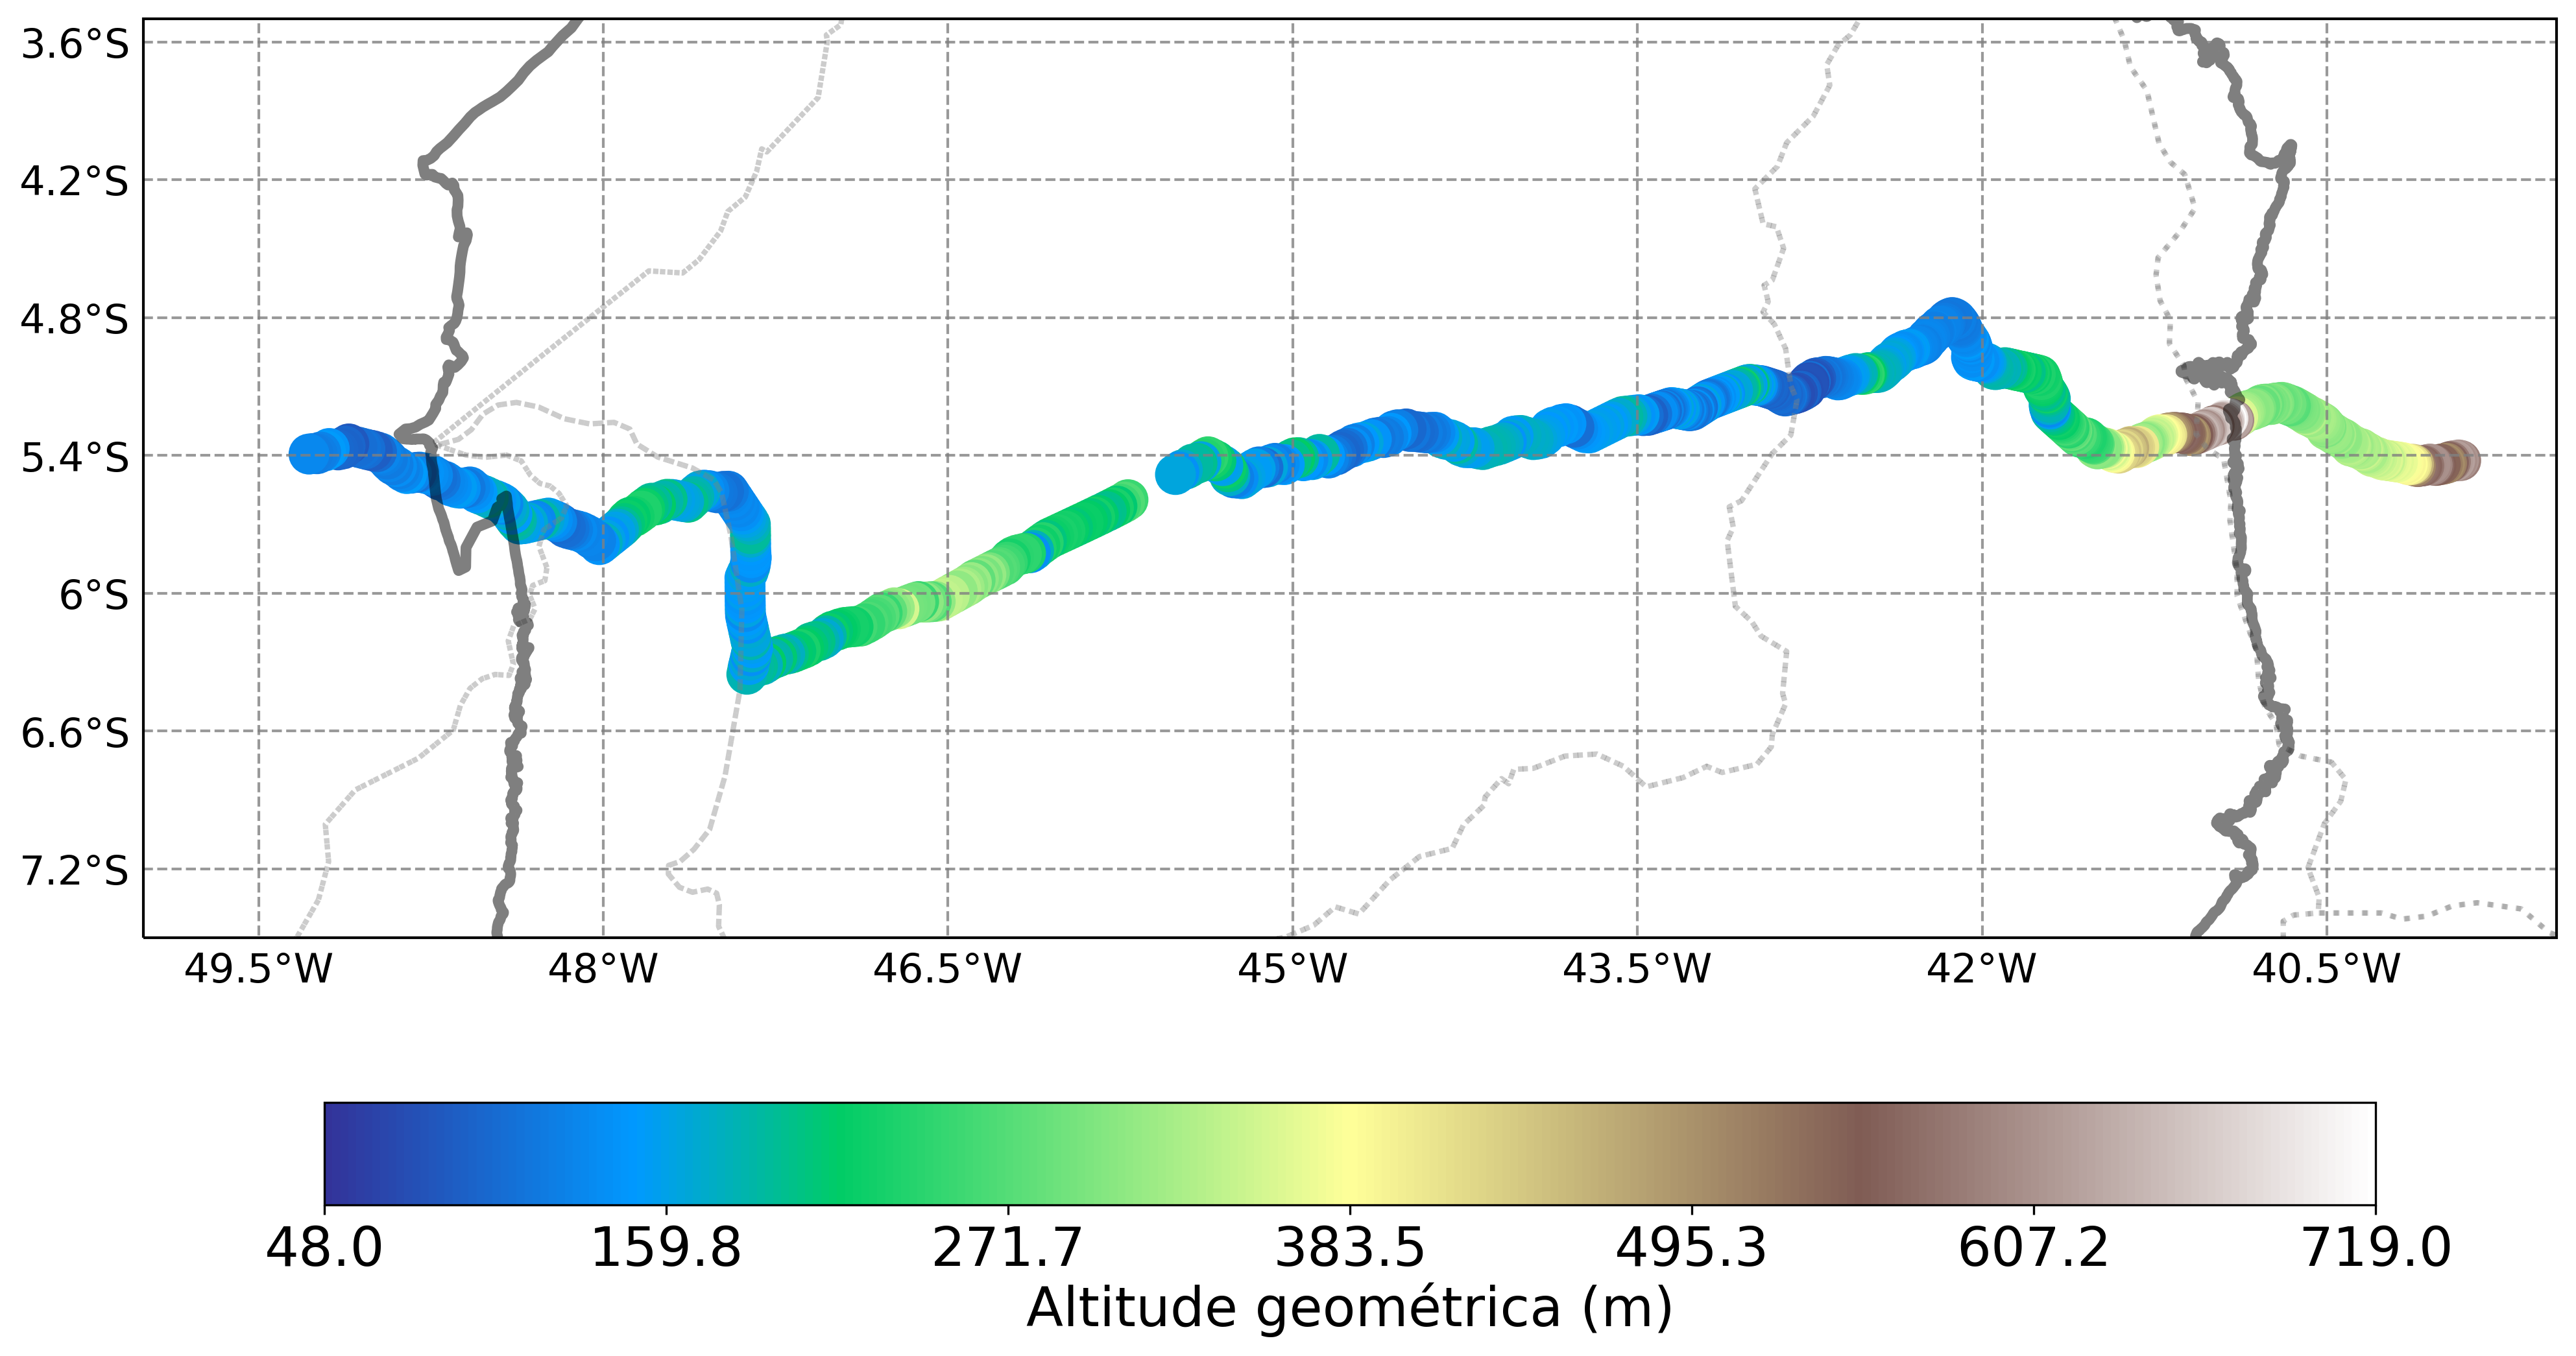
\includegraphics[scale=0.37]{figs/altitude geom campo.png}}
	\qquad
	\subfloat[Mapa com valores de $h$ preditos, pelo funcional \textit{h\_topo\_over\_ell}, apresentando uma variação de $48$ $m$ a $719$ $m$ metros de acordo com a escala de cores.]{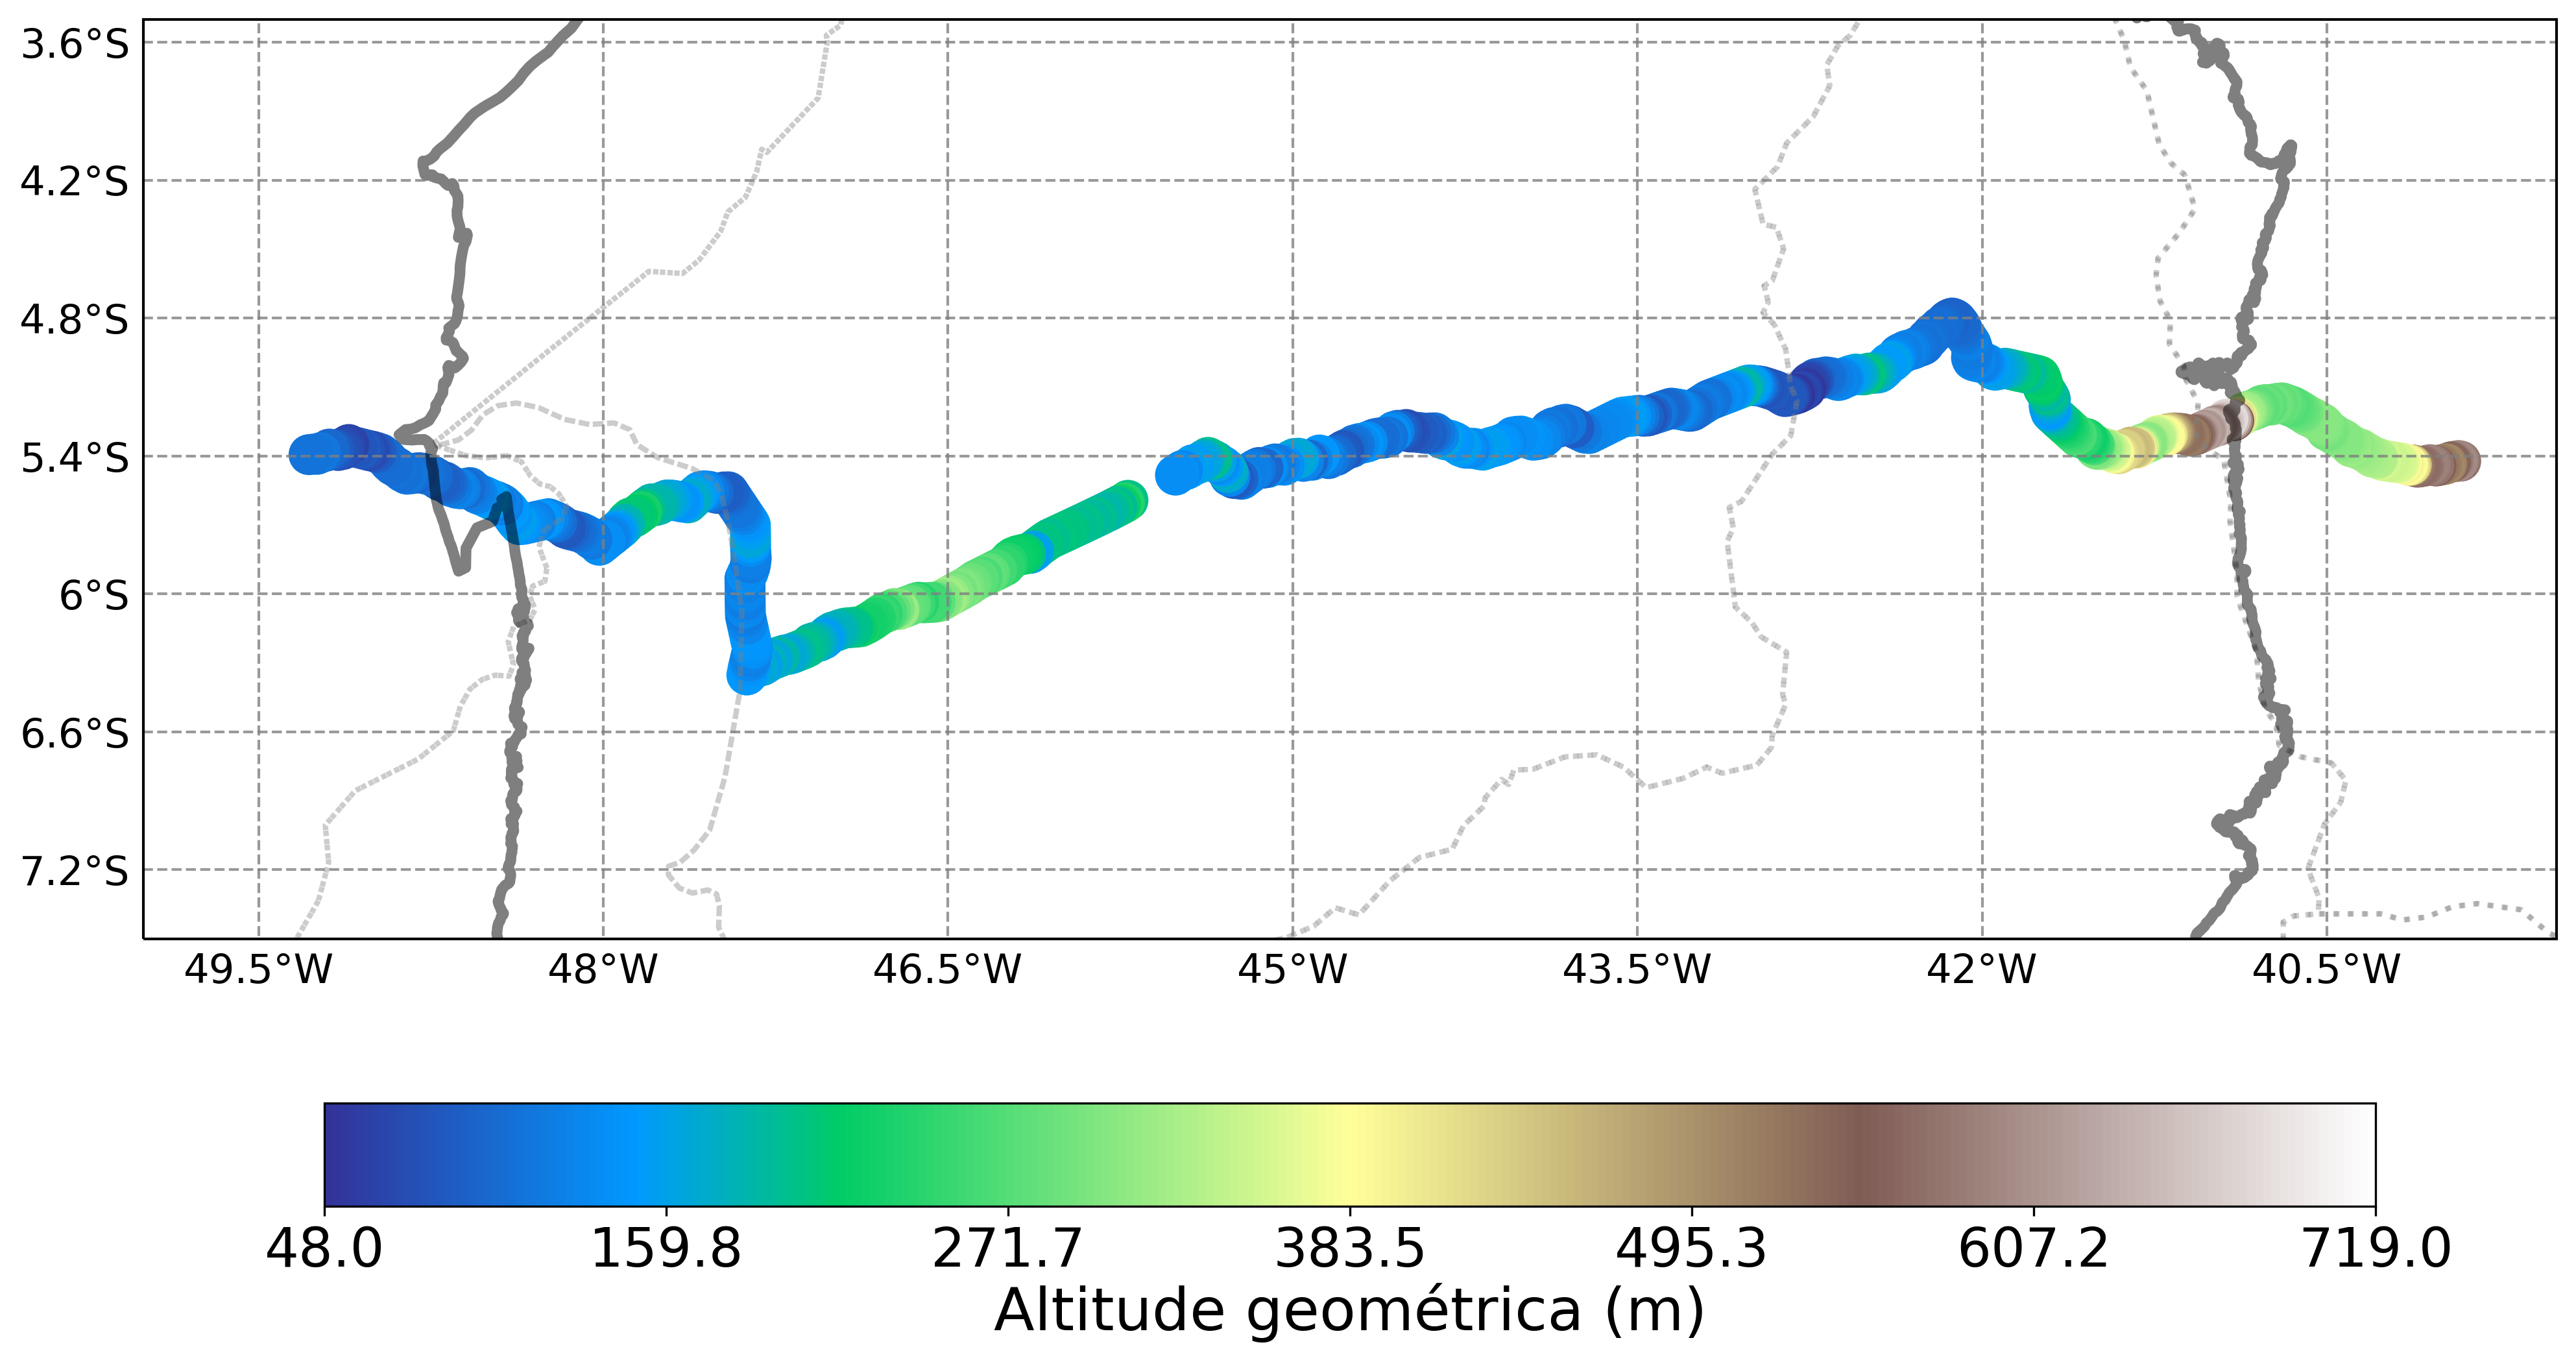
\includegraphics[scale=0.37]{figs/altitude geom predita campo.png}}% É possível observar certa similaridade nas altimetrias das diferentes metodologias.]{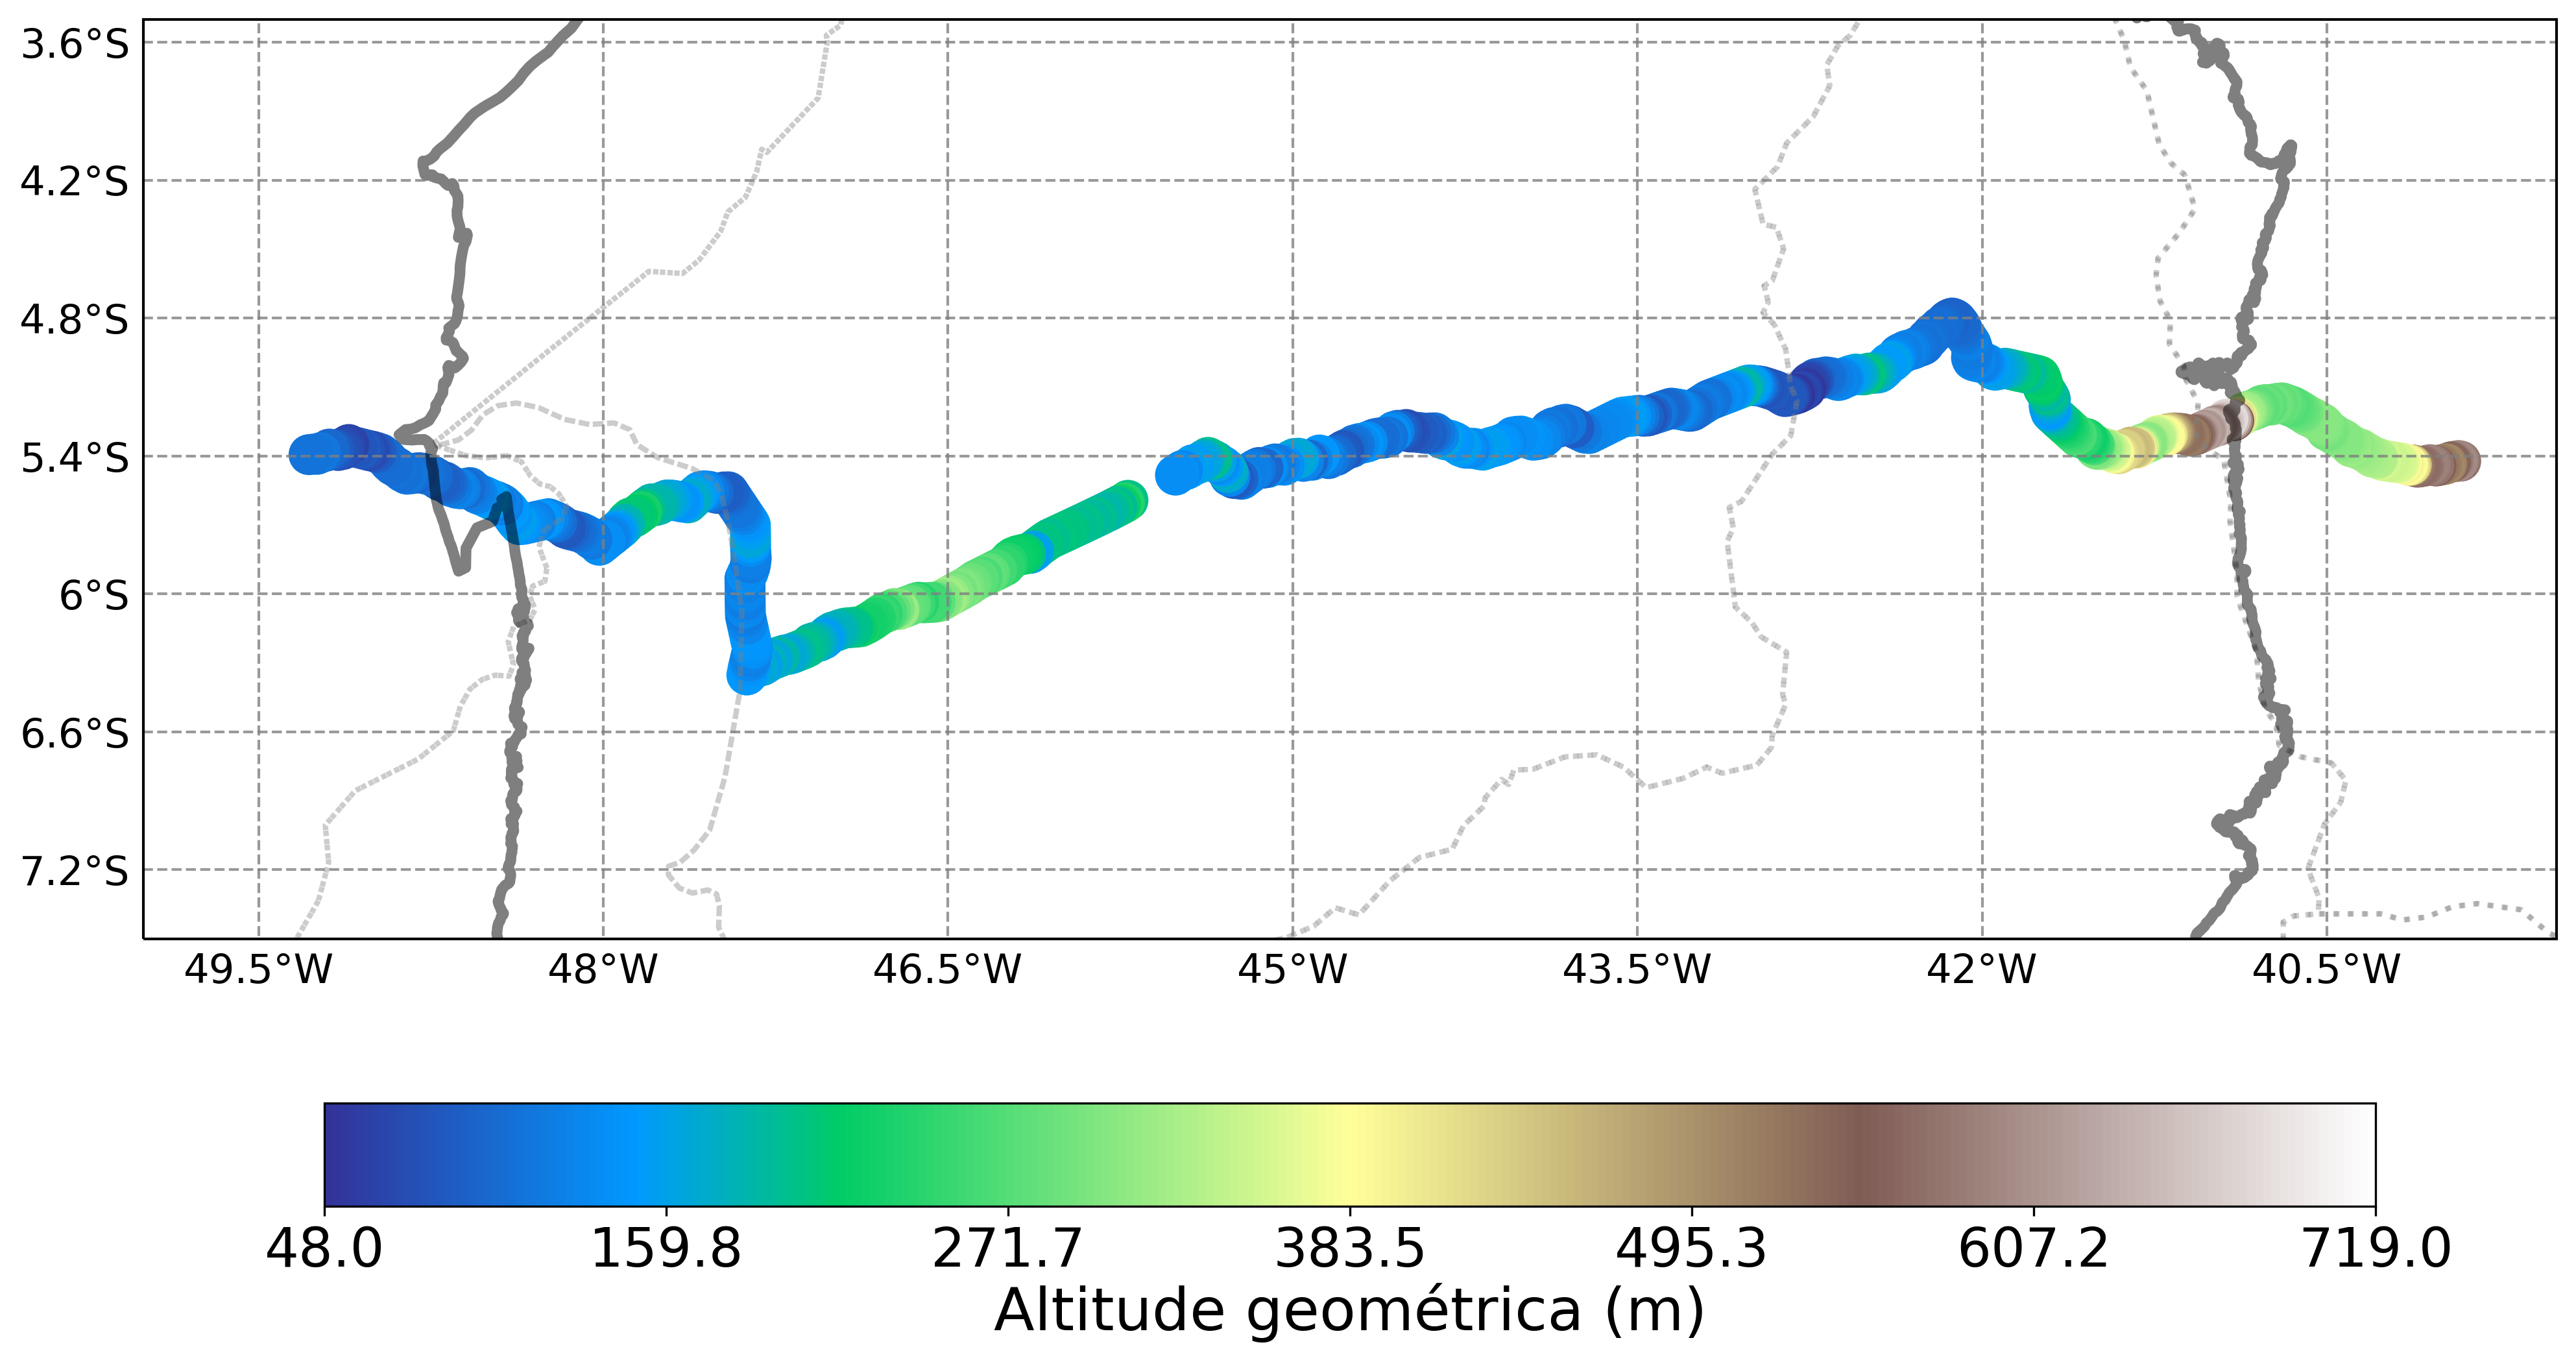
\includegraphics[scale=0.34]{figs/altitude geom predita campo.png}}
	\qquad
	\subfloat[Mapa de resíduos de $h$, calculados através da diferença entre $h$ observado e predito. com valores variando $\pm62.5$ $m$ segundo a escala de cores.]{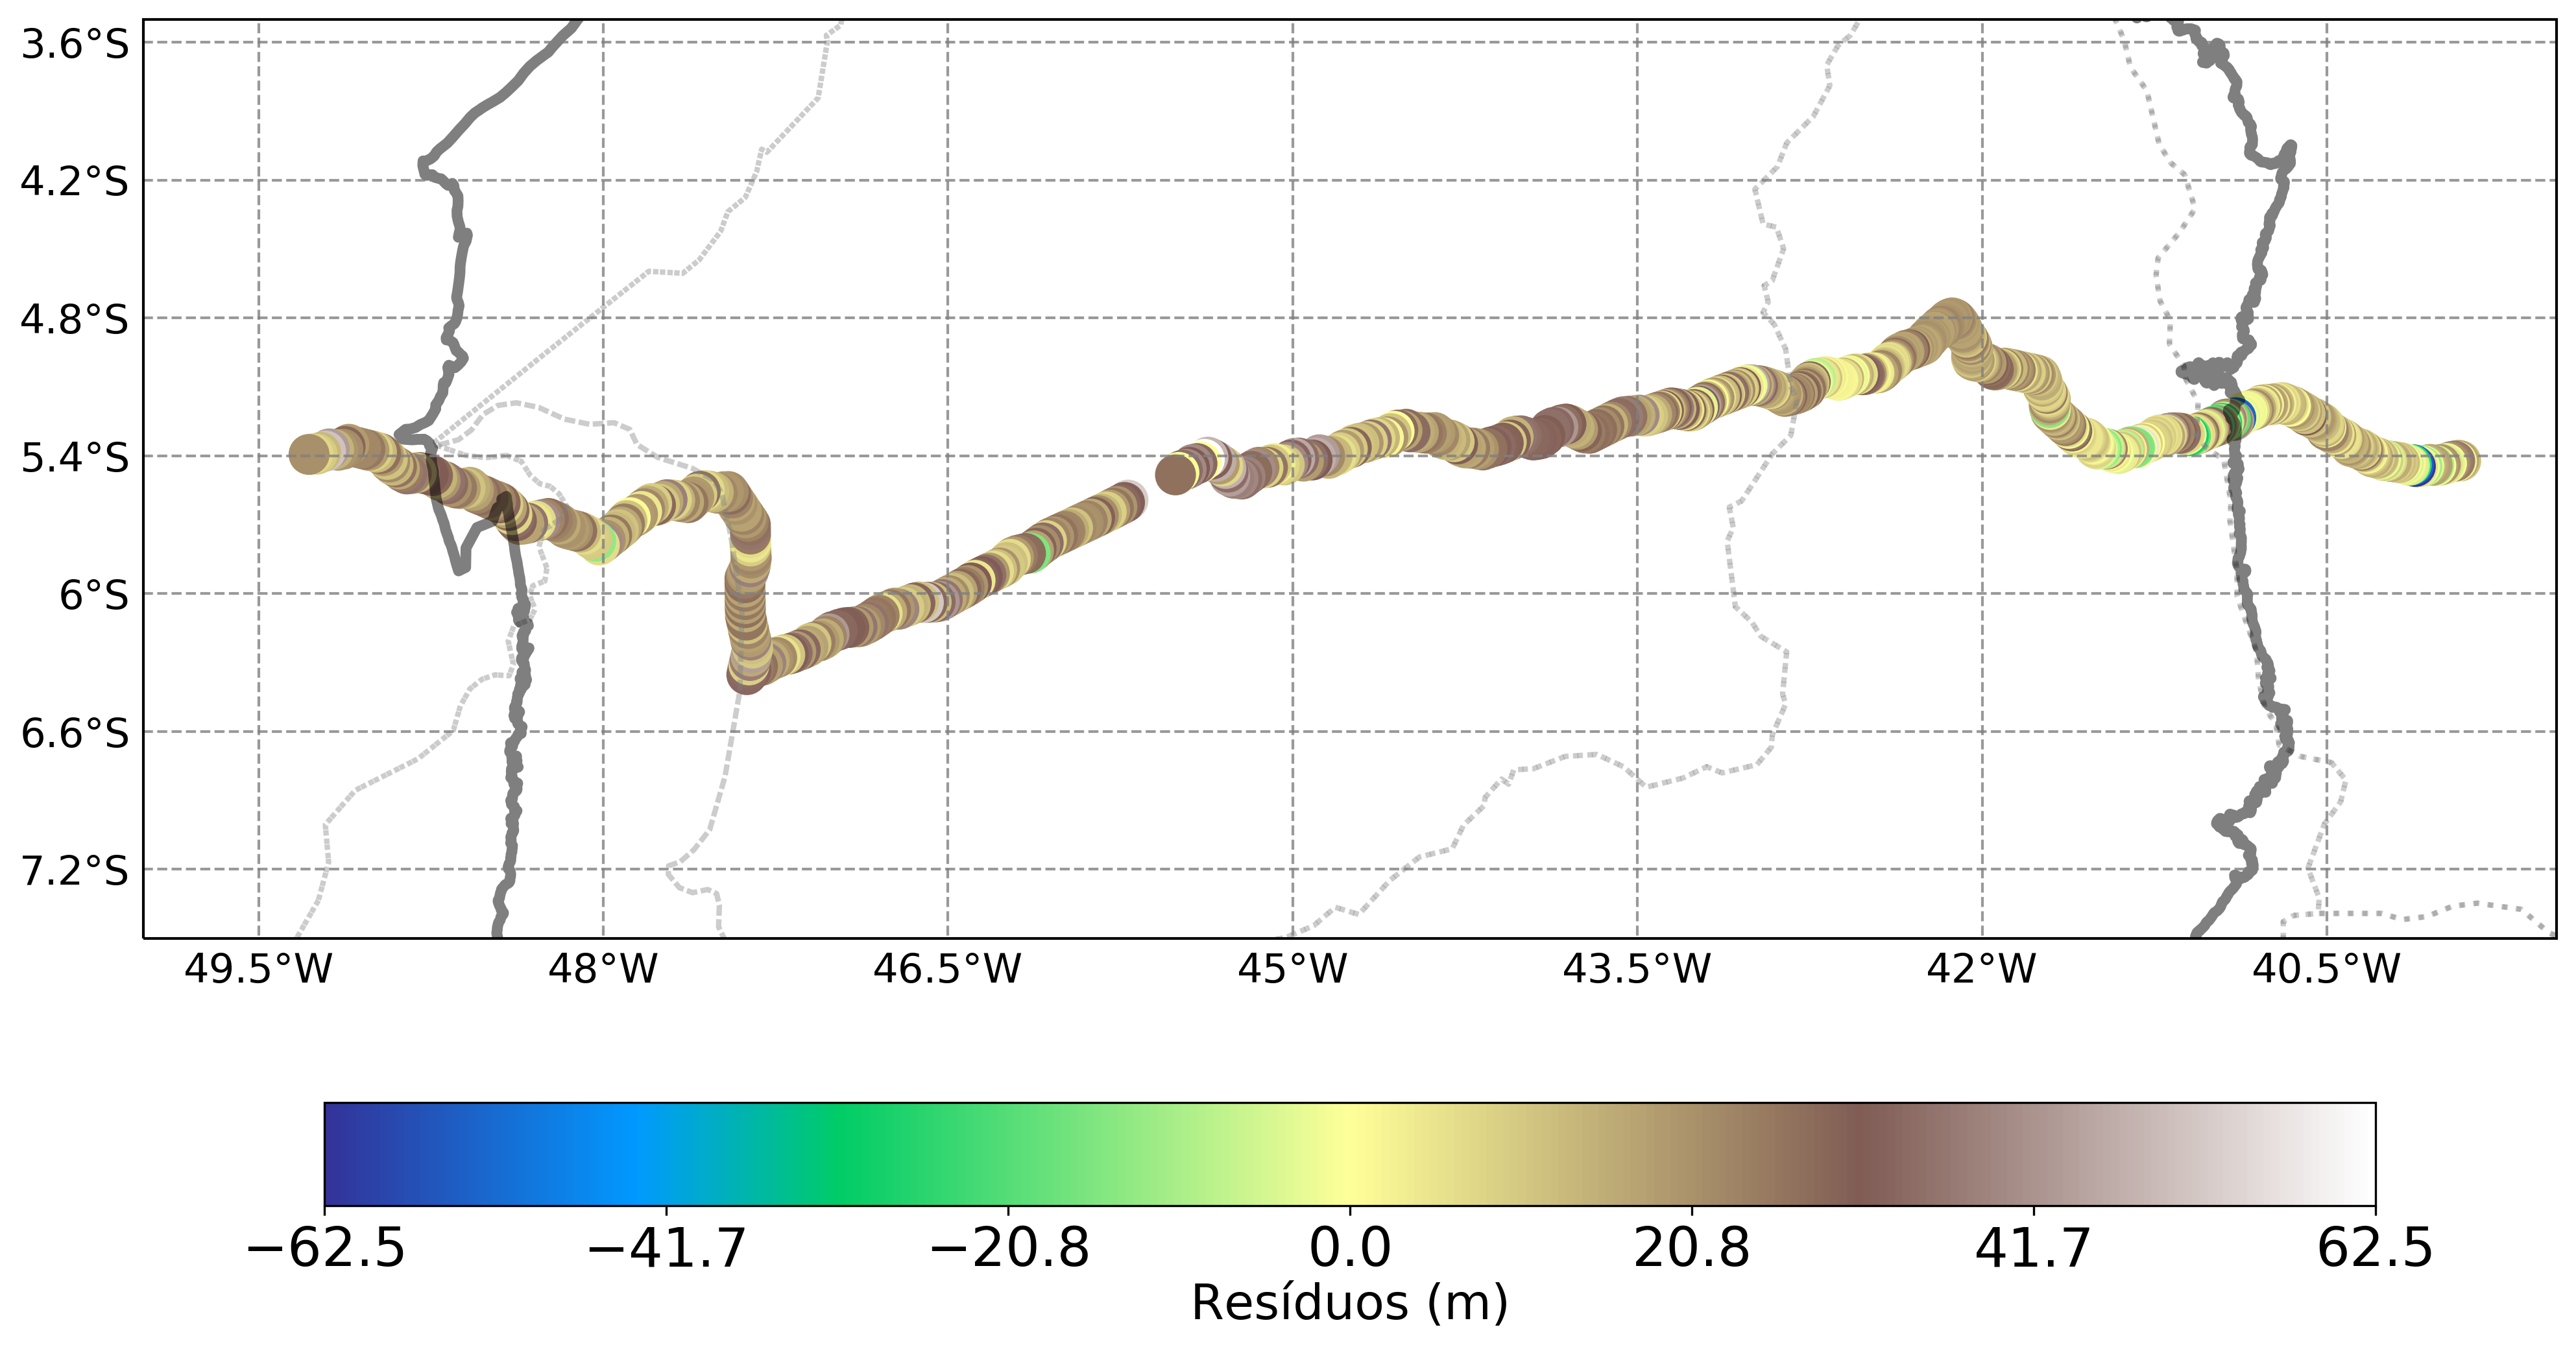
\includegraphics[scale=0.37]{figs/residuos altitude geom.png}} %Apresenta uma predominância positiva nos valores dos resíduos, possibilitando inferir que os dados preditos estão subestimados em relação aos dados observados.]{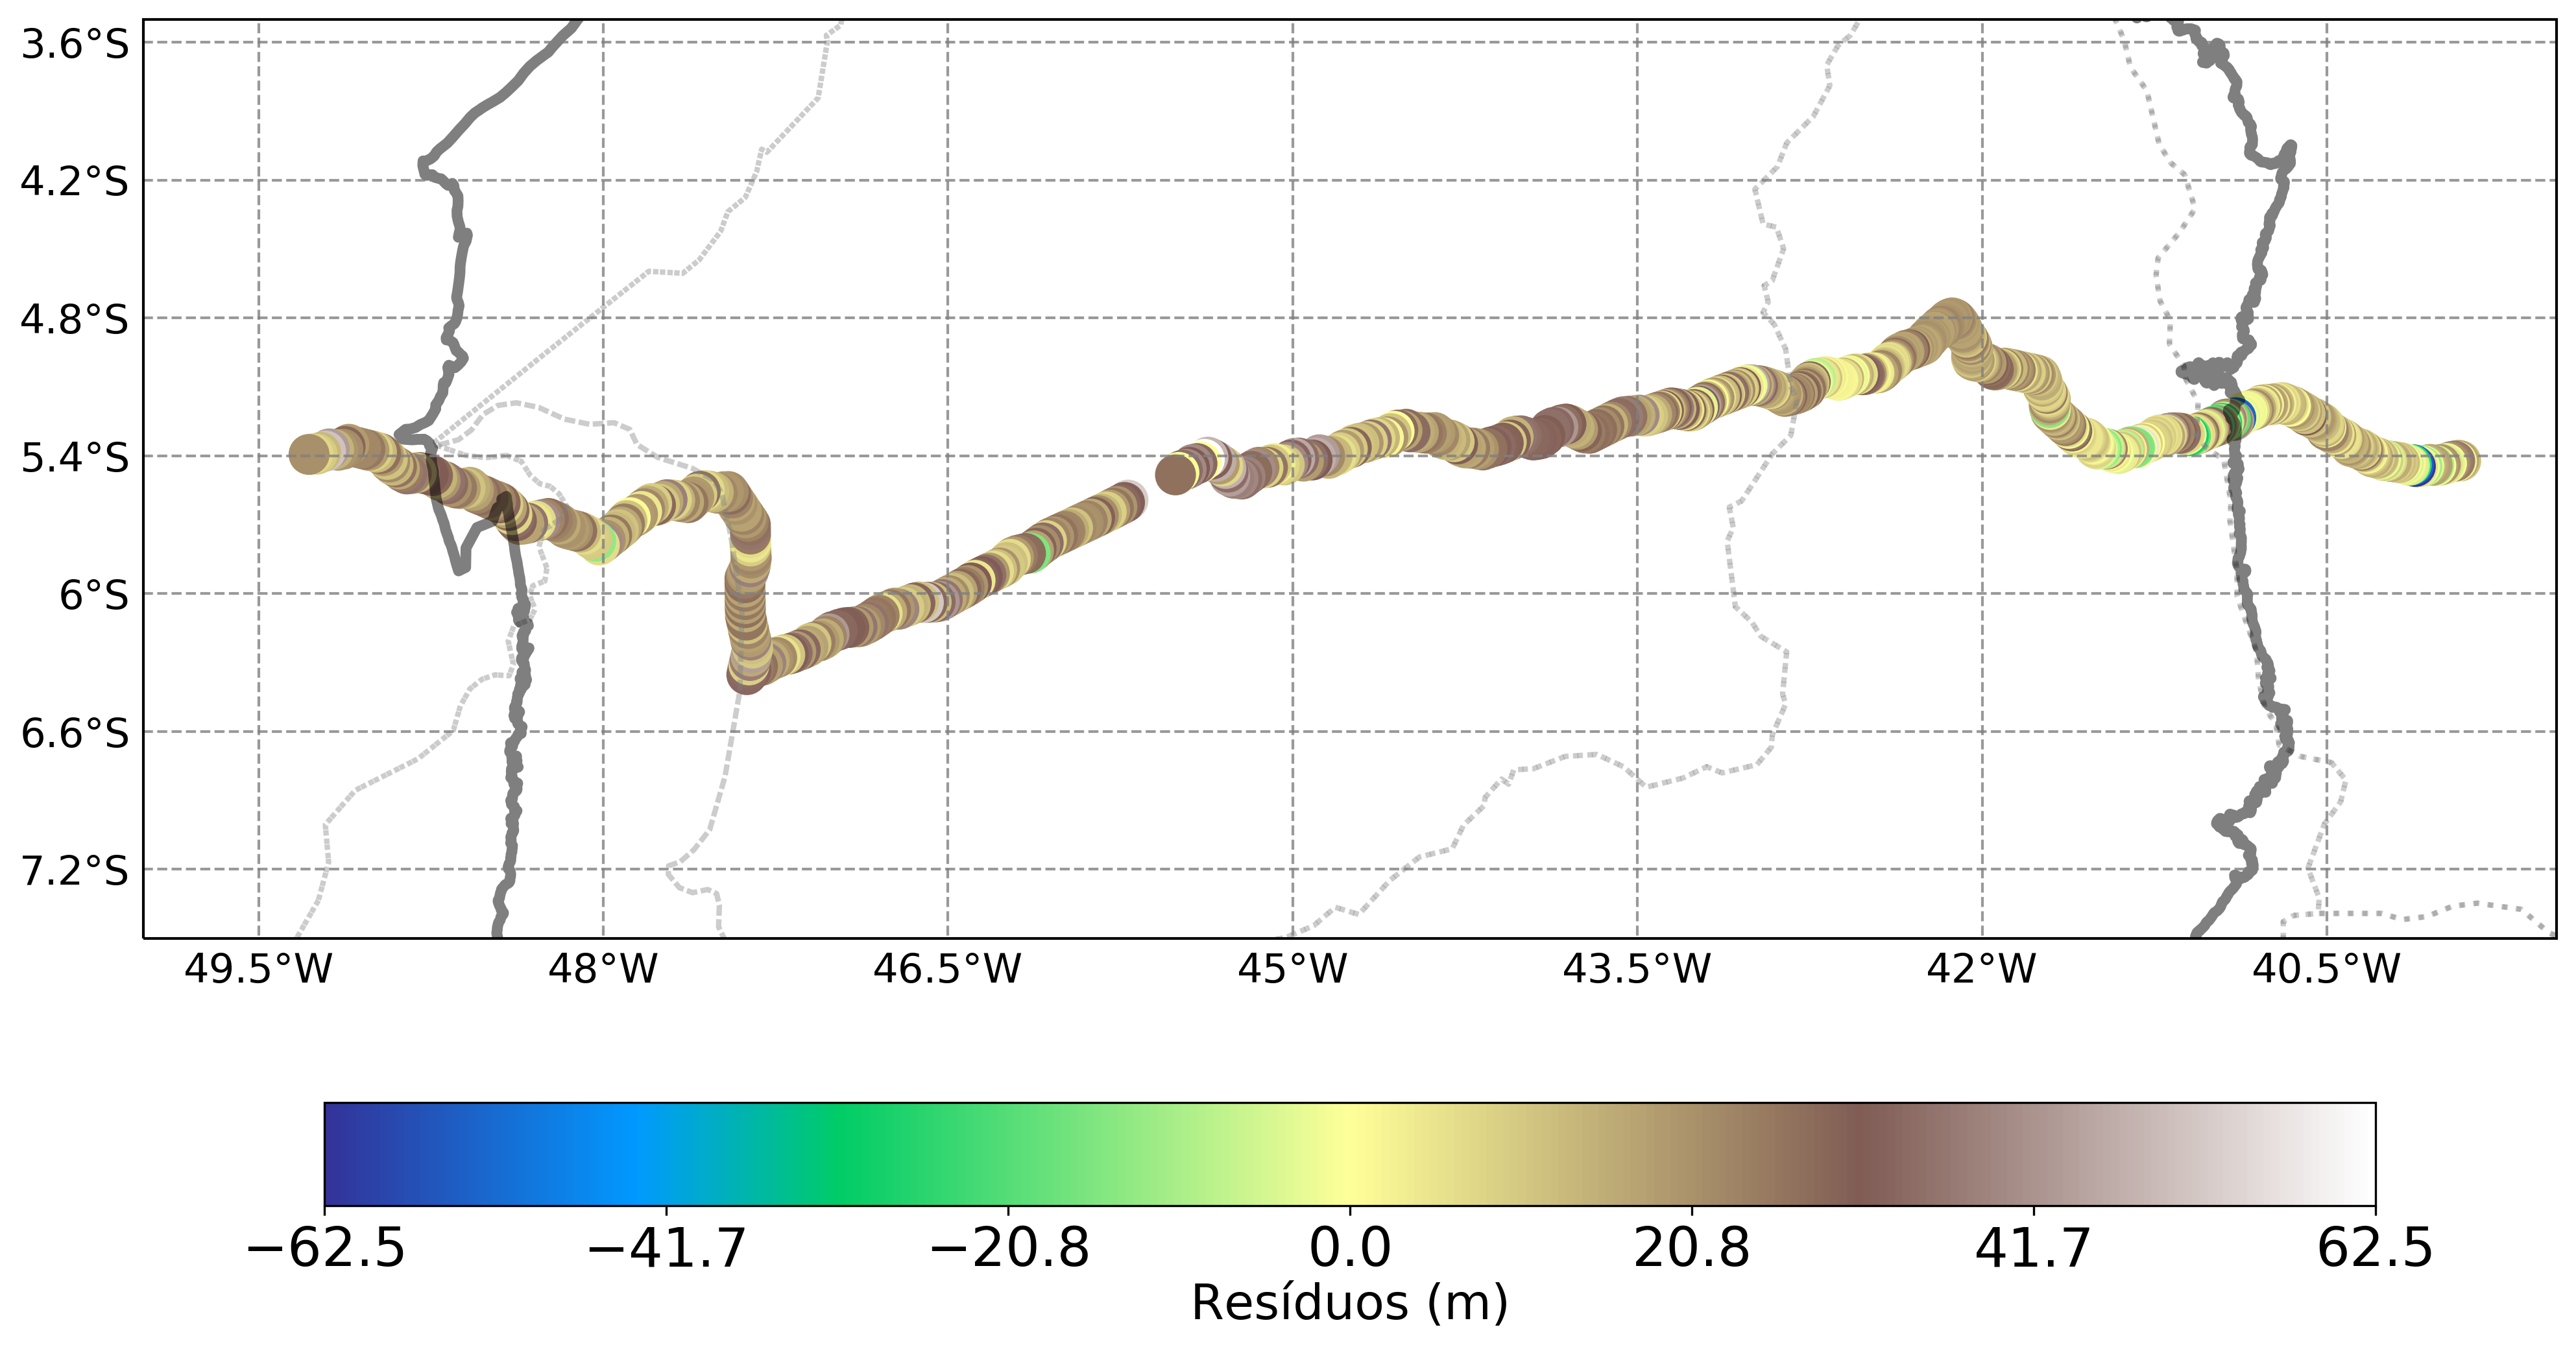
\includegraphics[scale=0.34]{figs/residuos altitude geom.png}}
	\caption{Esquema comparativo de $h$ observado, $h$ predito e os resíduos de $h$ como objeto de comparação. O contorno preto representa os limites da bacia do Parnaíba, e o contorno cinza, o limite dos estados.}  
	\label{subfig:residuos_h}
\end{figure}

Os resíduos de $h$ apresentaram valores majoritariamente positivos, que se repetem com maior frequência  entre as faixas amarela e marrom, segundo a escala de cores, que corresponde à faixa de $0$ à $\approx25$ metros. Essa análise leva à hipótese de que os dados preditos estão subestimados em relação aos observados. É provável que seja resultado do truncamento dos harmônicos esféricos, visto que é necessário impor um trucamento para interromper a expansão em determinado grau e ordem. Para complementar a hipótese da subestimativa de $h$, foi gerado o histograma dos resíduos apresentado na Figura \ref{subfig:histograma_h}.a. Pode-se observar que a média é igual a $17.38$m e desvio padrão de $12.70$m, em que se destaca o comportamento majoritariamente positivo dos resíduos. Essa análise evidencia um erro de tendência. O gráfico de correlação da Figura \ref{subfig:histograma_h}.b entre as altitudes geométricas observadas e preditas apontam para uma região mais densa de pontos para $h$ menor que $400$m, enquanto que para valores mais altos há uma dispersão, aparentemente,  um pouco maior. Isto não prejudica os resultados, já que é possível constatar uma boa correlação linear com o coeficiente de determinação ($R^{2}$) igual à $0.99,$ o que mostra que $h$ predito se ajusta linearmente ao observado com $99$\% de eficácia. No entanto, é preciso levar em conta que a amostragem dos dados tem pouca cobertura em pontos com amplitudes altimétricas maiores. 

\begin{figure}[H]
	\centering
	\subfloat[Histograma dos resíduos de $h$, onde é possível observar um comportamento na média de $17,38$ metros e desvio padrão igual a $12.7$. A linha vermelha pontilhada corresponde ao histograma de resíduo teórico, considerando uma distribuição gaussiana.]{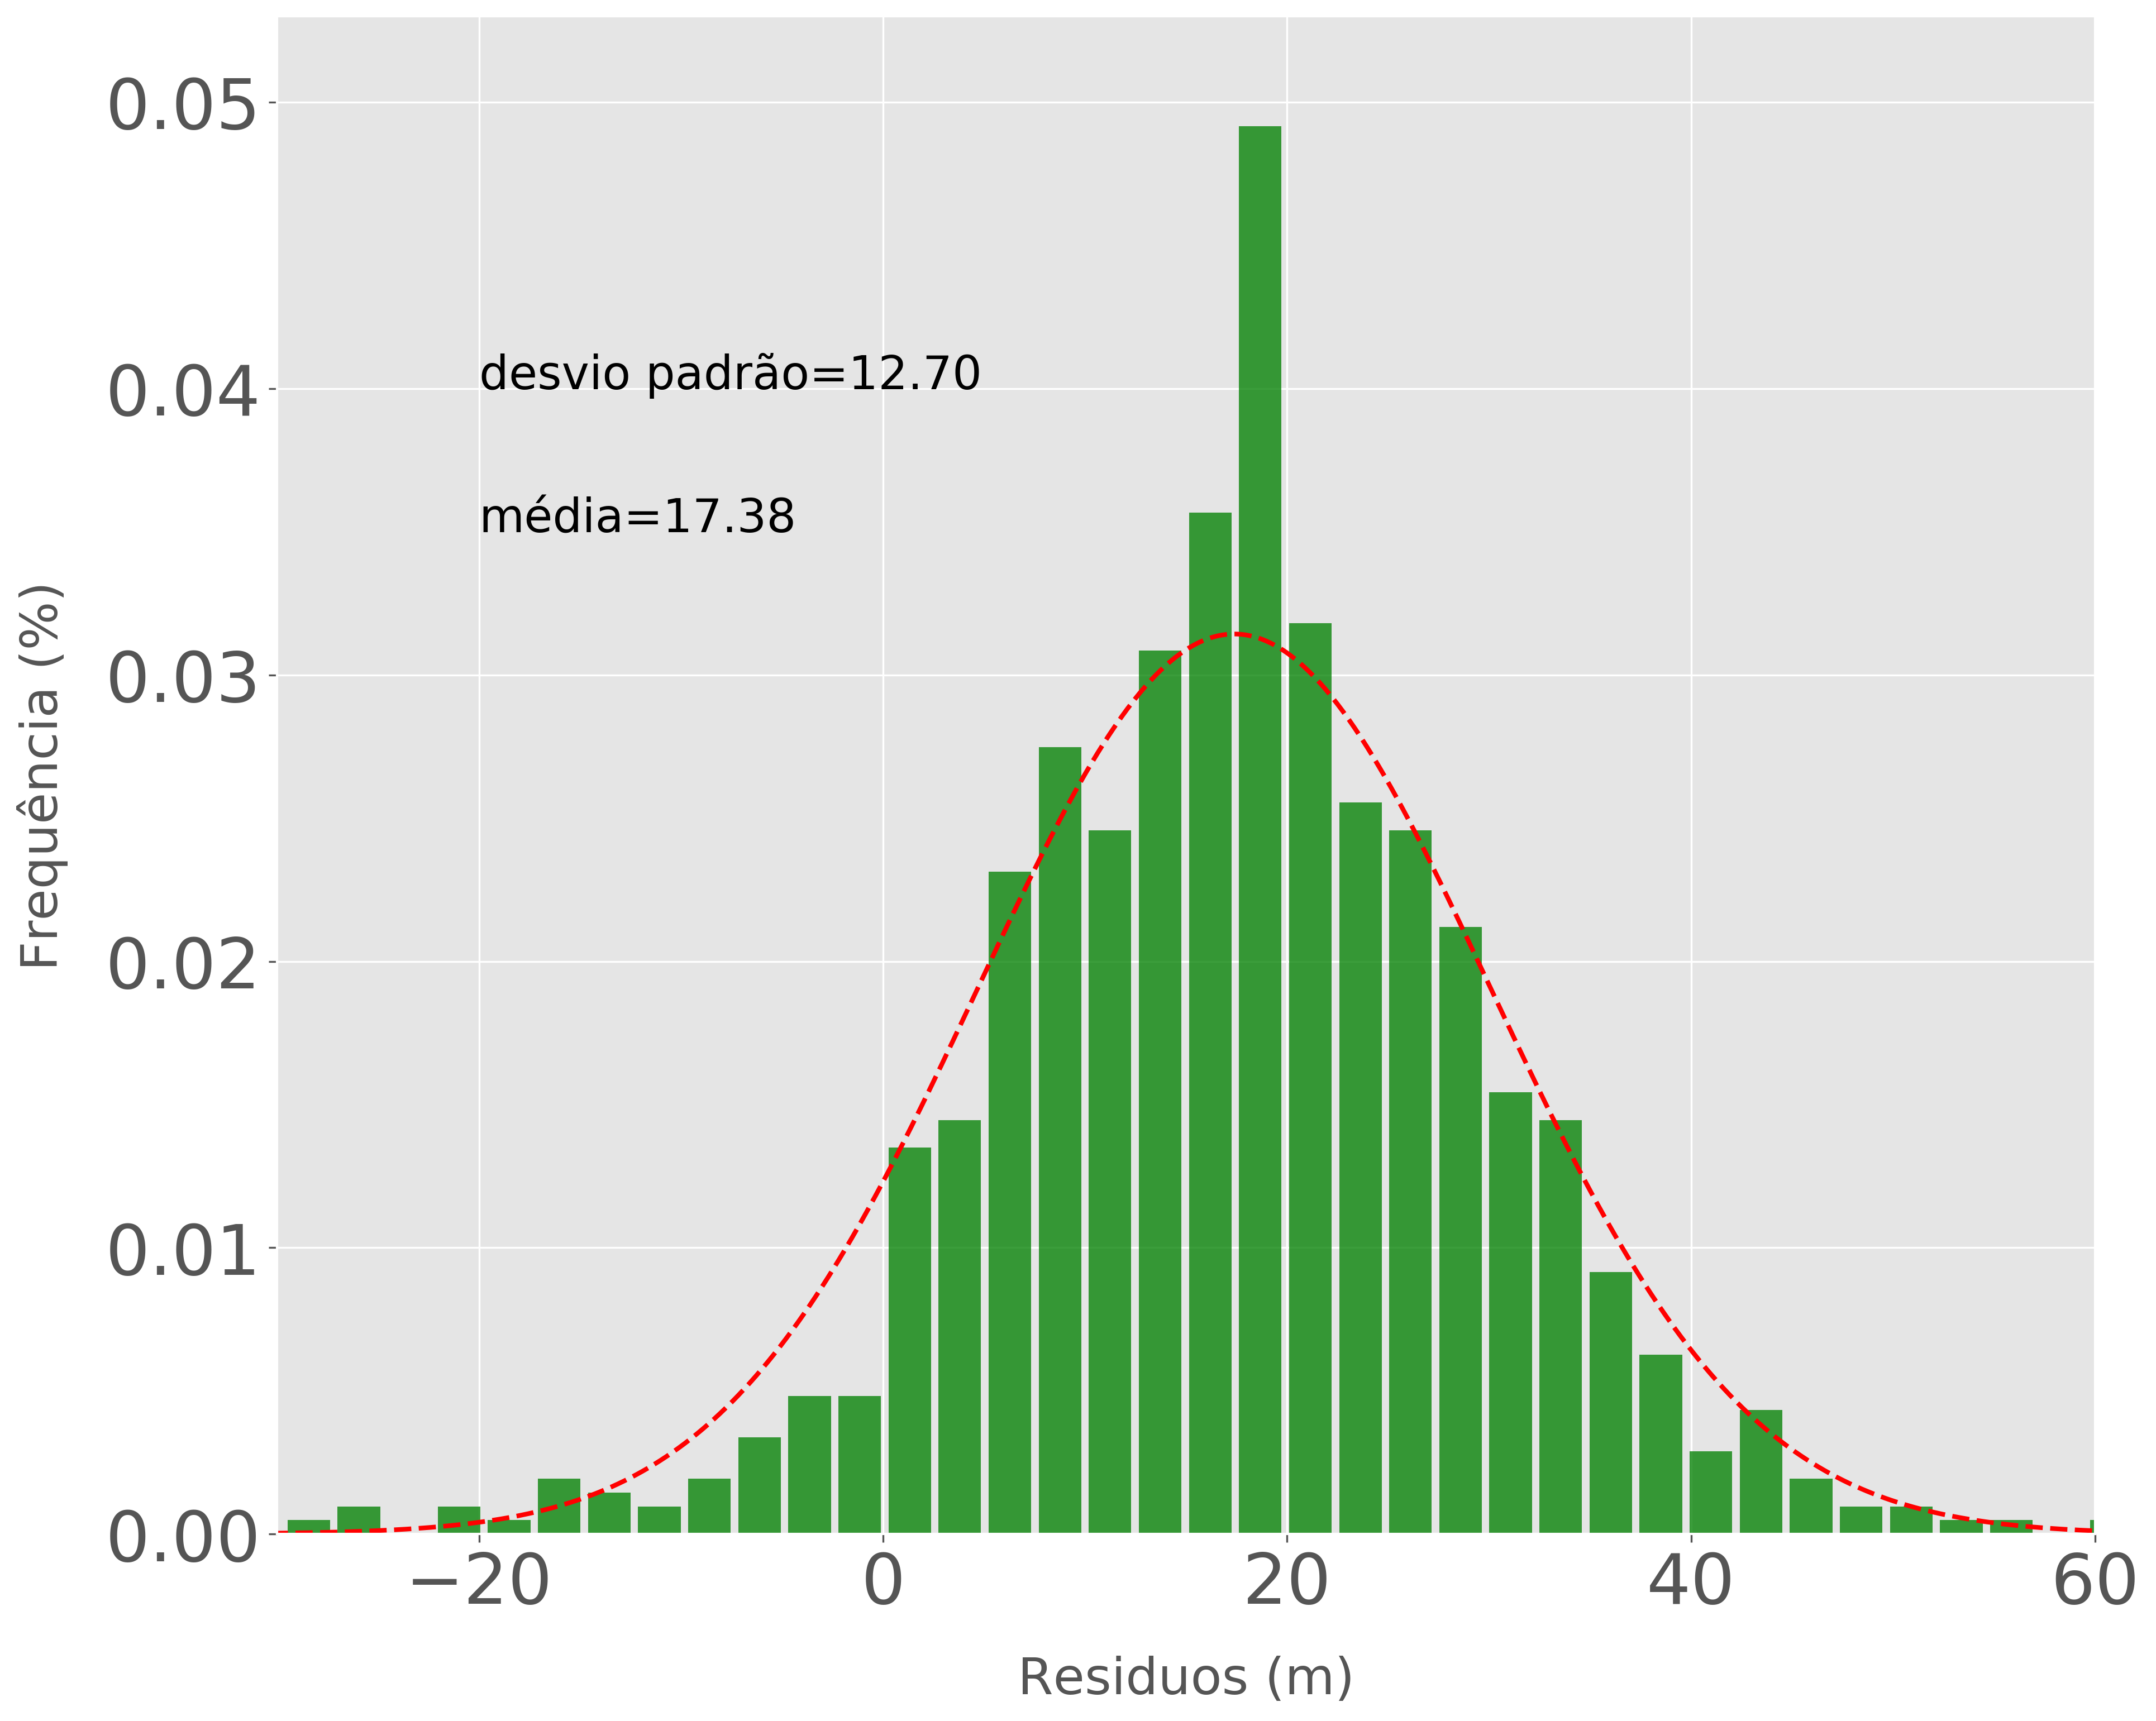
\includegraphics[scale=0.245]{figs/histograma_residuos_h.png}}
	\ 
	\,\,\subfloat[Gráfico de dispersão de $h$, observado e predito, com ajuste linear representado pela reta vermelha com $R^{2}$ igual à $0,99$.]{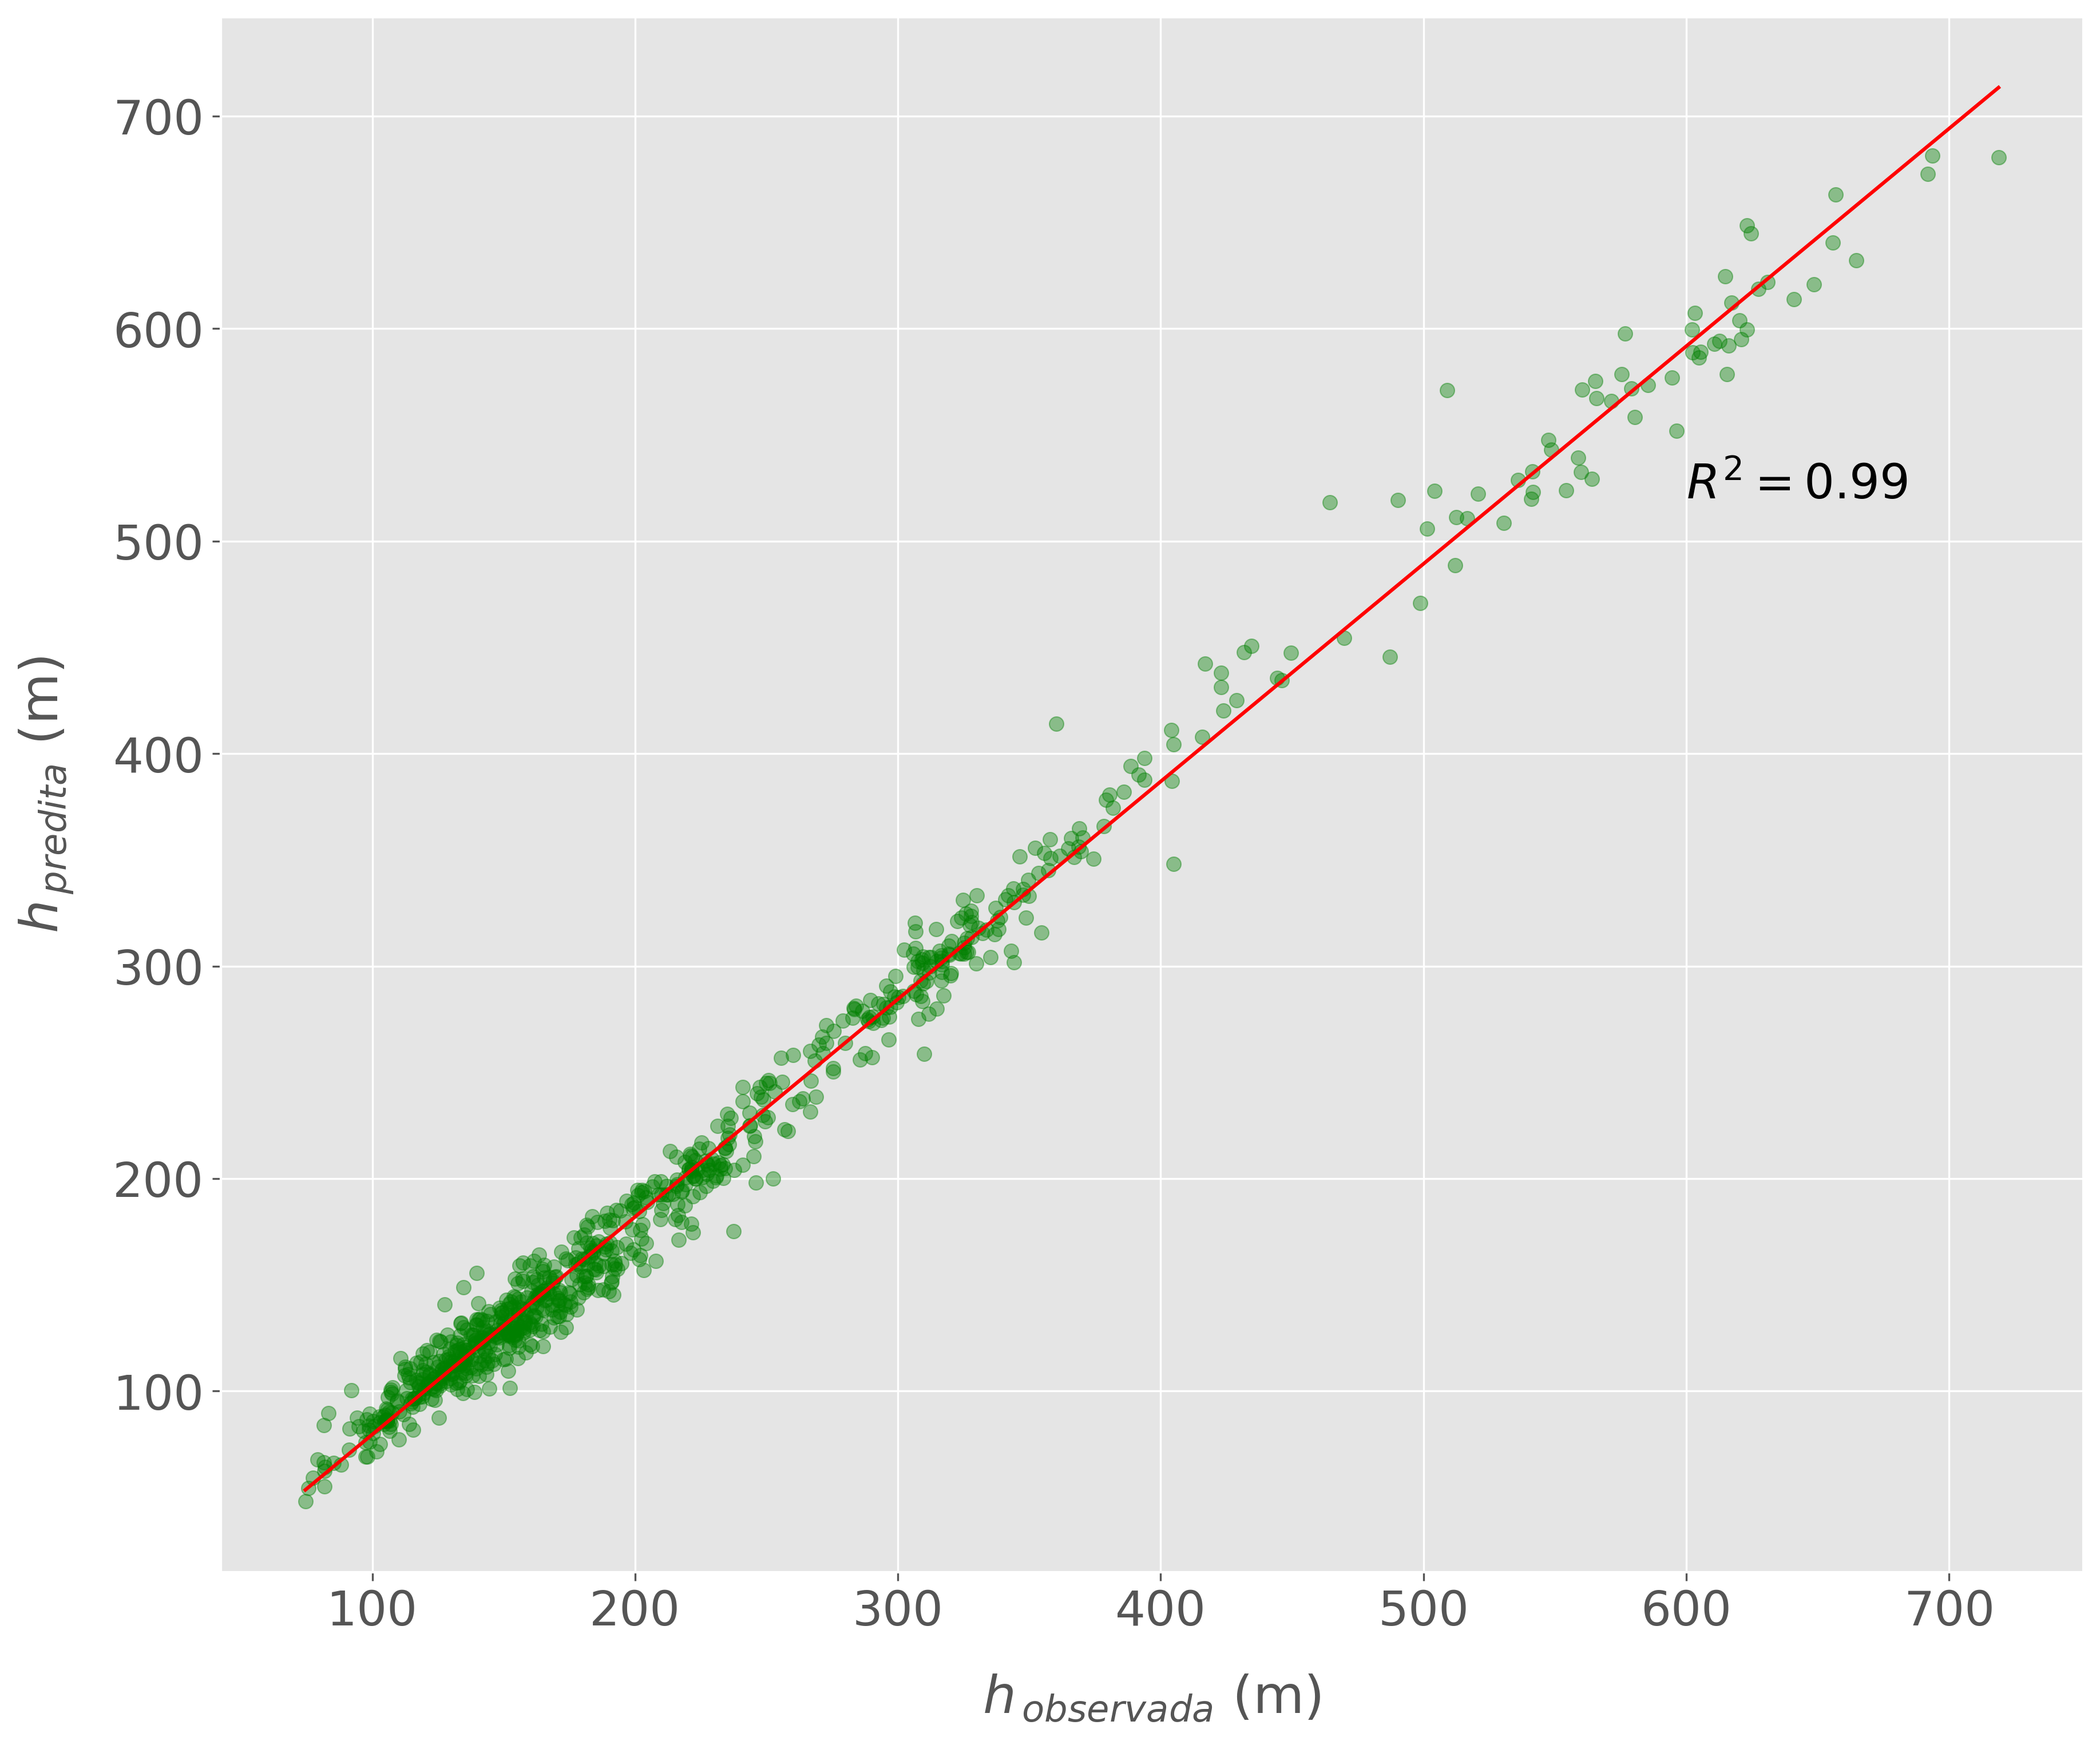
\includegraphics[scale=0.245]{figs/dispersao h obs x pred.png}}
	\caption{Esquema com histograma de resíduos de $h$ ao lado do gráfico de correlação $h$, observado e predito.}  
	\label{subfig:histograma_h}
\end{figure}


\section{Distúrbio de gravidade ($\delta g$)}

Assim como nas análises altimétricas, foram geradas imagens para analisar $\delta g$ da região da bacia do Parnaíba. A Figura \ref{fig:comparacao_delta} compreende a sobreposição das estações gravimétricas do levantamento à malha regular obtida por satélite no fundo da imagem. Ambas retratam valores de $\delta g$ dentro da escala de cores definida, variando em $\pm70.0$ $mGal$. É possível observar um contraste nos valores de $\delta g$, principalmente na borda leste em relação à porção central, sendo o meio da bacia majoritariamente negativo, fato que já era esperado para uma bacia sedimentar. Destaca-se também que esse padrão tem uma certa correlação com aquele mostrado na Figura \ref{fig:comparacao_h} referente a $h$. Através da análise dos padrões observados e preditos é possível constatar boa similaridade entre as diferentes metodologias de aquisição de dados, terrestre e de satélite. Todavia, nota-se que alguns pontos apresentam valores levemente diferentes de $\delta g$ observados em comparação com os preditos. Sendo assim, foram aplicados os mesmos procedimentos realizados durante a análise de $h$ para $\delta g$. A Figura \ref{subfig:residuos_delta}.a e .b apresenta, para cada estação gravimétrica, os distúrbios observados e preditos, respectivamente. A escala de cores é igual em todos os gráficos, variando em $\pm57$ $mGal$. É possível constatar uma conformidade geral, mas, assim como no caso das altitudes geométricas, existem incongruências pontuais entre os distúrbios, como na região entre $42$º$W$ e $43.5$º$W$, e na região entre $45$º$W$ e $46.5$º$W$. A diferença entre os distúrbios pode ser vista no mapa da Figura \ref{subfig:residuos_delta}.c que corresponde ao resíduos obtidos. Esse mapa apresenta uma variação de $\pm 22.5$ $mGal$. 


\begin{figure}[H]
	\centering
	\includegraphics[scale=0.47]{figs/disturbio obs X pred.png}
	\caption{Imagem de $\delta g$ da região da Bacia do Parnaíba, sendo o contorno preto os limites desta, e o contorno pontilhado em cinza, o limite dos estados. Ao fundo, $\delta g$ predito pela malha regular gerada a partir dos valores de gravidade absoluta calculados pelo funcional \textit{gravity earth} e gravidade normal calculados pela fórmula analítica da gravidade, através da equação \ref{eq:disturbio}; sobrepondo, na forma do caminhamento terrestre, são $\delta g$ observados.}
	\label{fig:comparacao_delta}
\end{figure}


\begin{figure}[H]
	\centering
	\subfloat[Mapa com valores de $\delta g$ observados, com variação de $\pm57$ $mGal$ de acordo com a barra de cores, obtidos através da equação \ref{eq:disturbio}.]{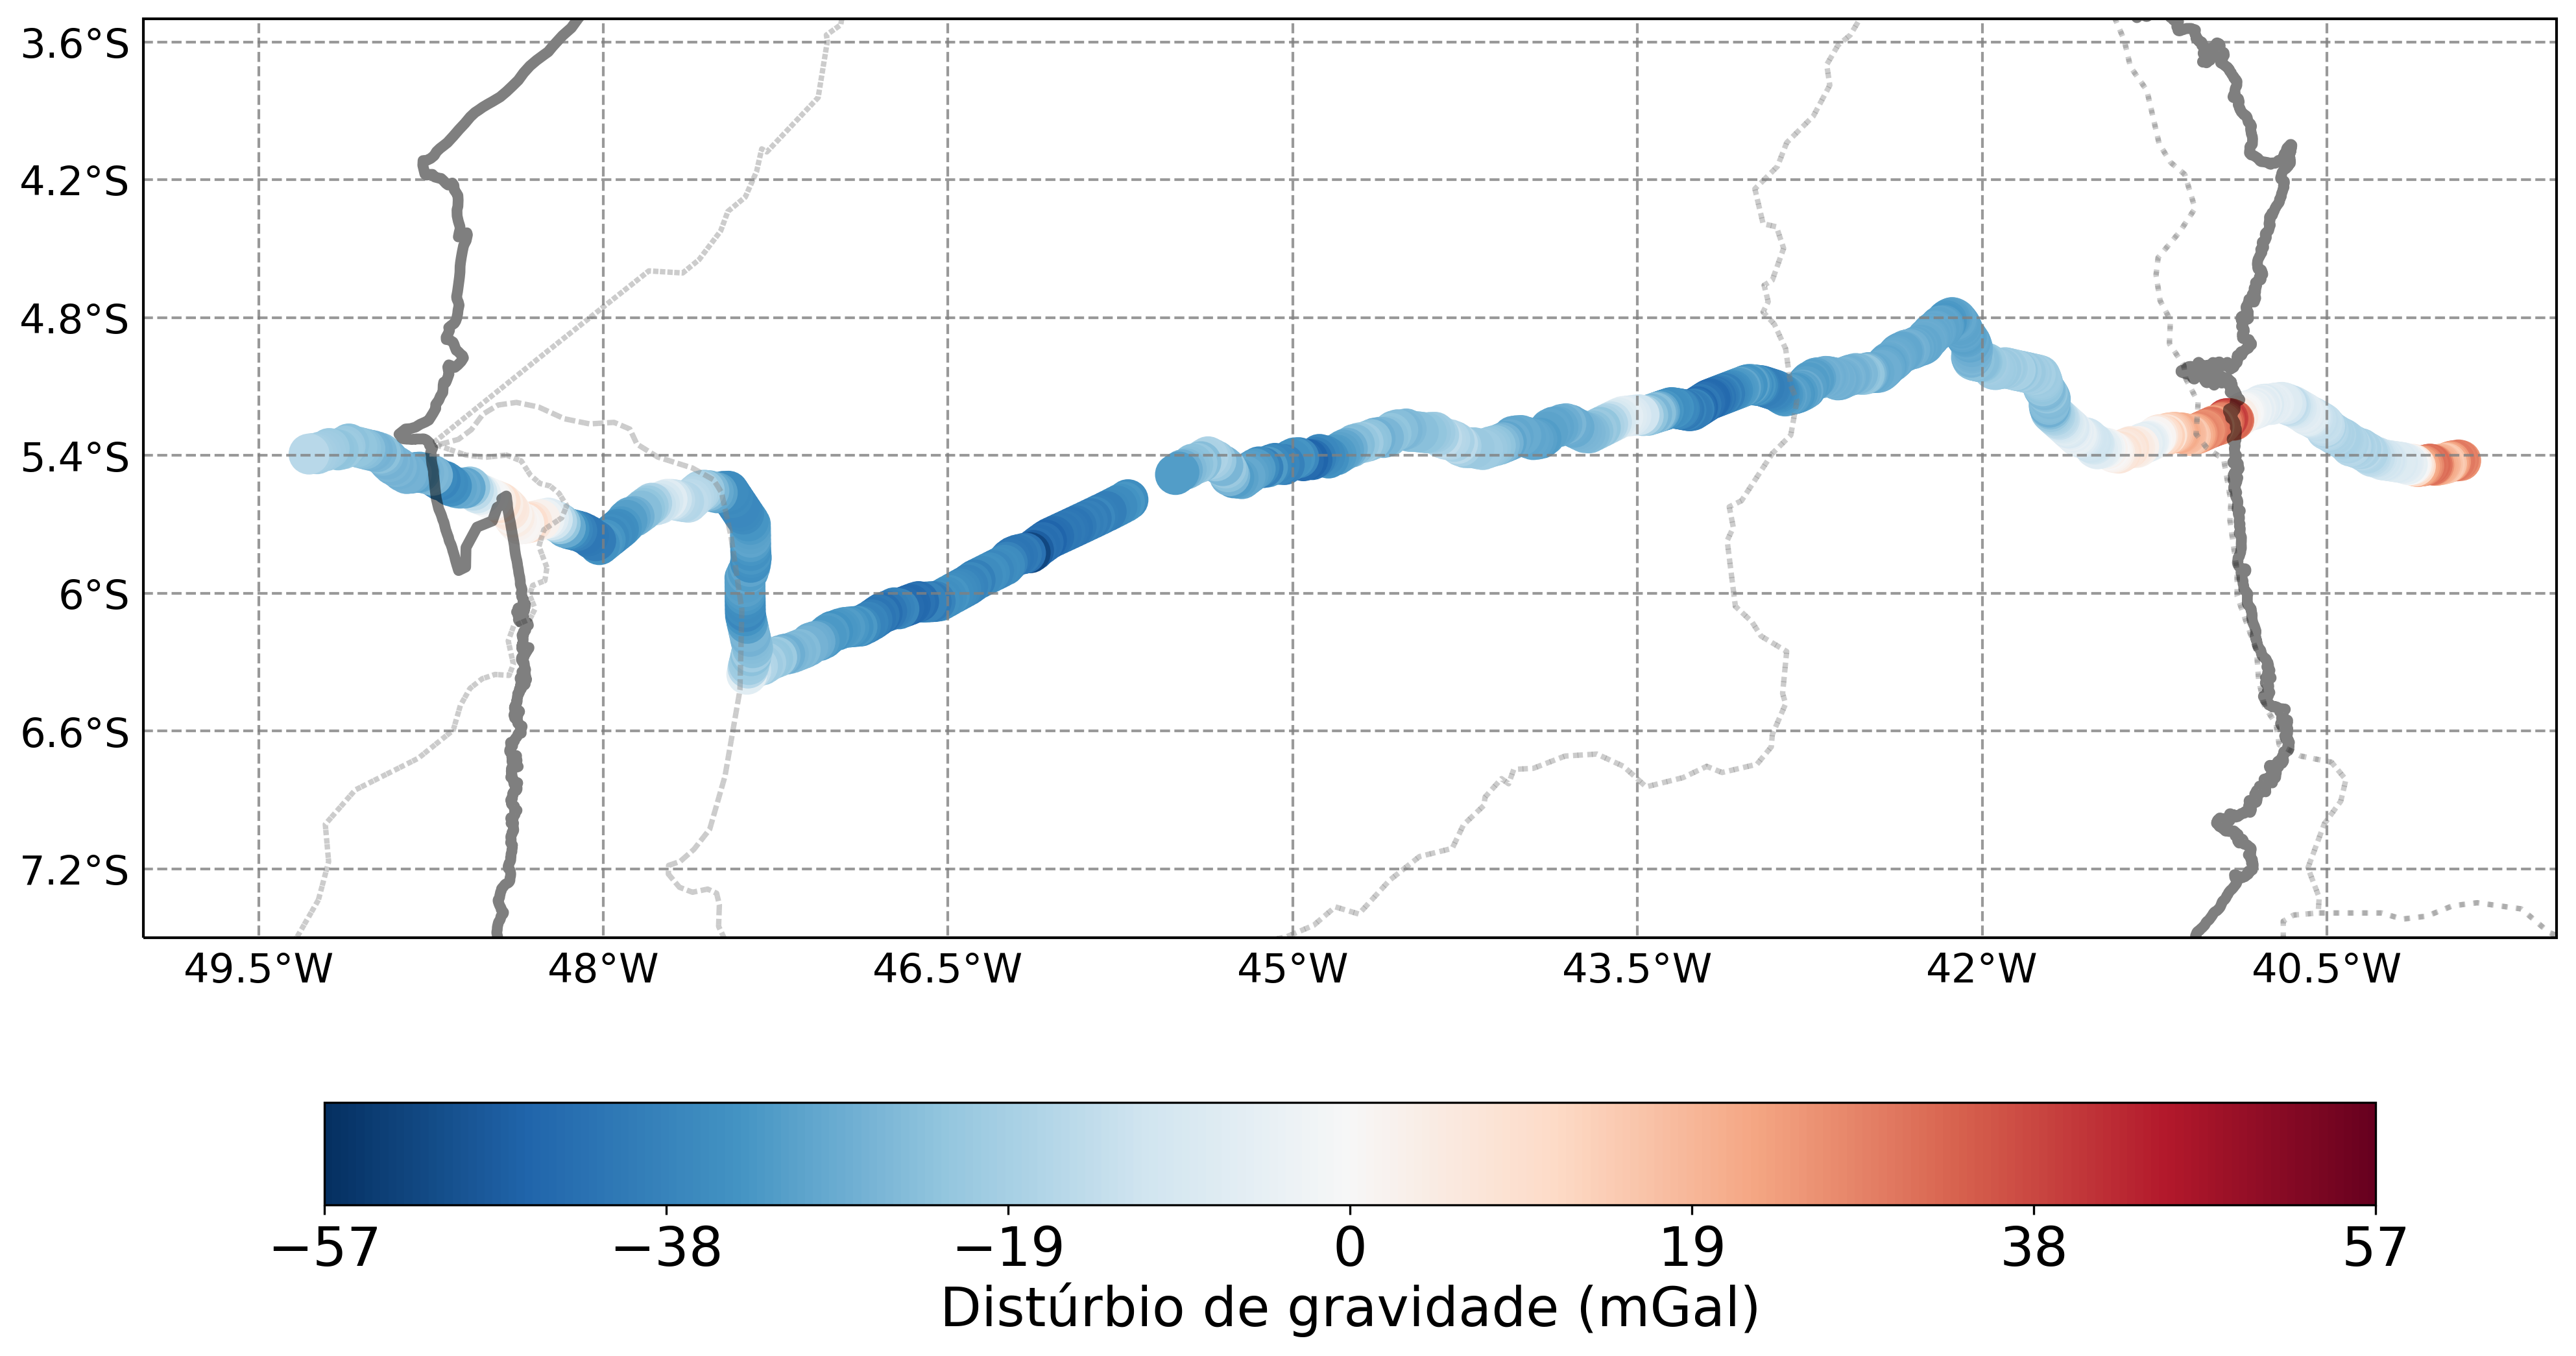
\includegraphics[scale=0.37]{figs/perfil disturbio observado.png}}
	\
	\subfloat[Mapa com valores de $\delta g$ preditos, com variação de $\pm57$ $mGal$ de acordo com a barra de cores, obtidos através da equação \ref{eq:disturbio}.]{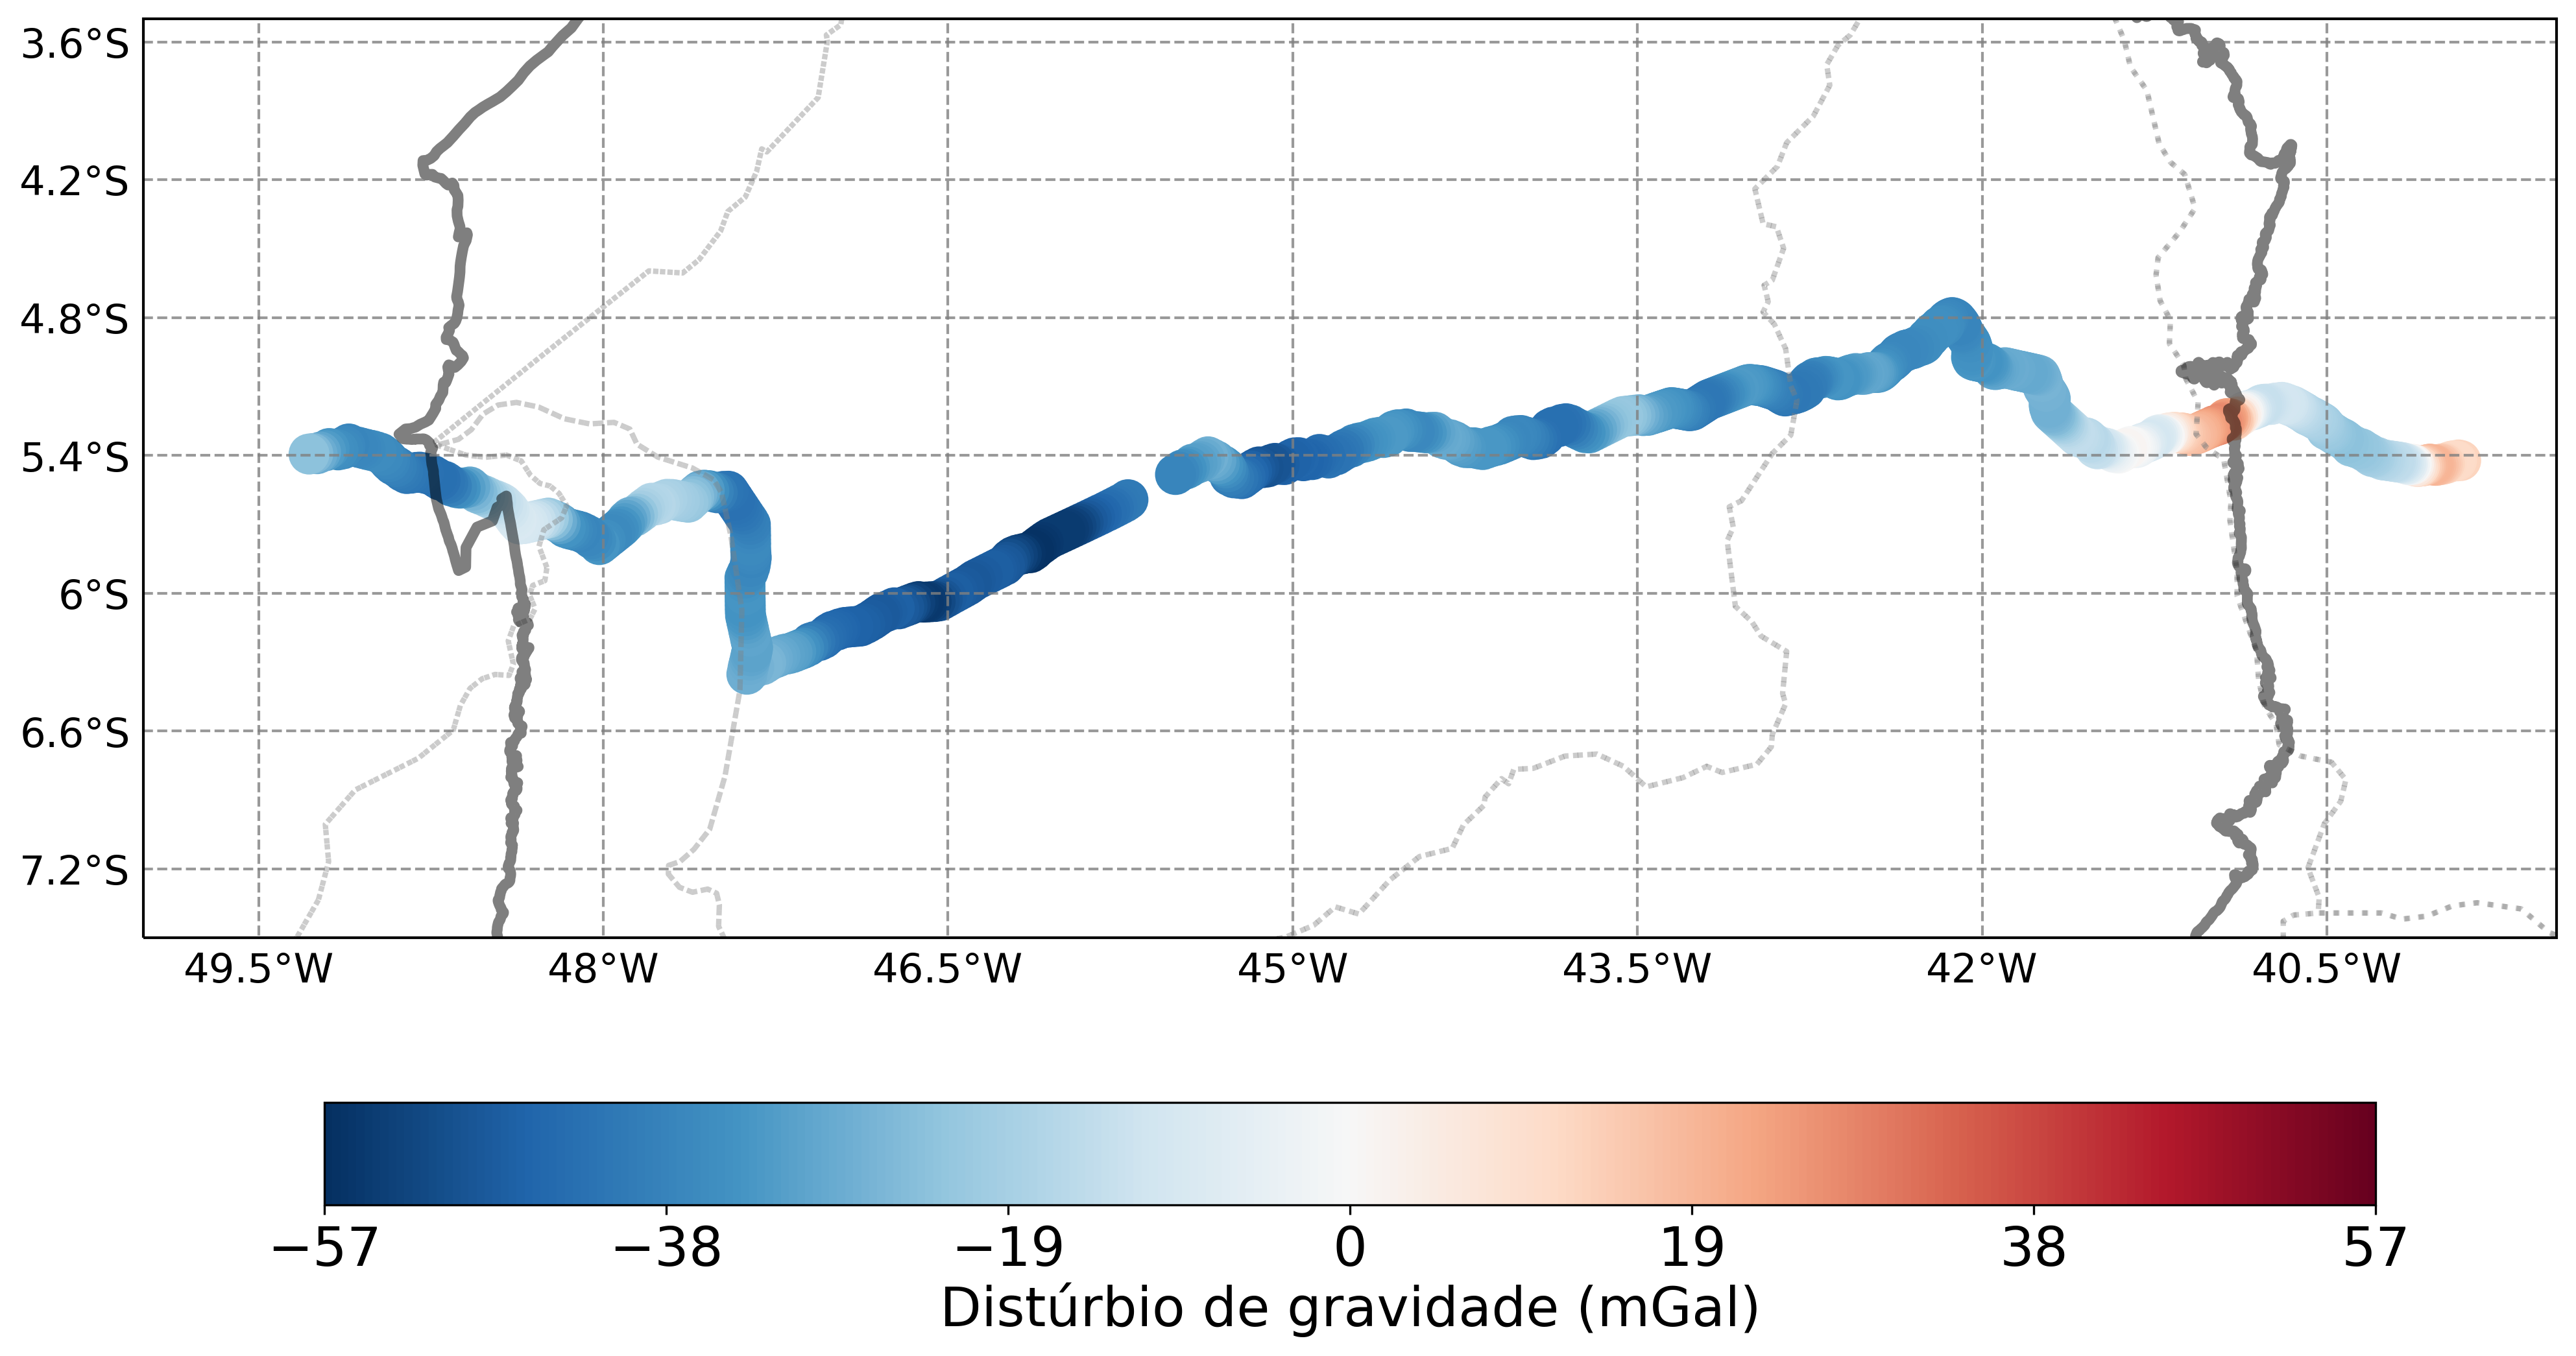
\includegraphics[scale=0.37]{figs/perfil disturbio predito.png}} 
	\
	\subfloat[Mapa de resíduo de $\delta g$ obtido pela diferença entre os distúrbios observados e preditos, apresentando uma variação de $\pm22.5$ $mGal$ de acordo com a escala de cores.]{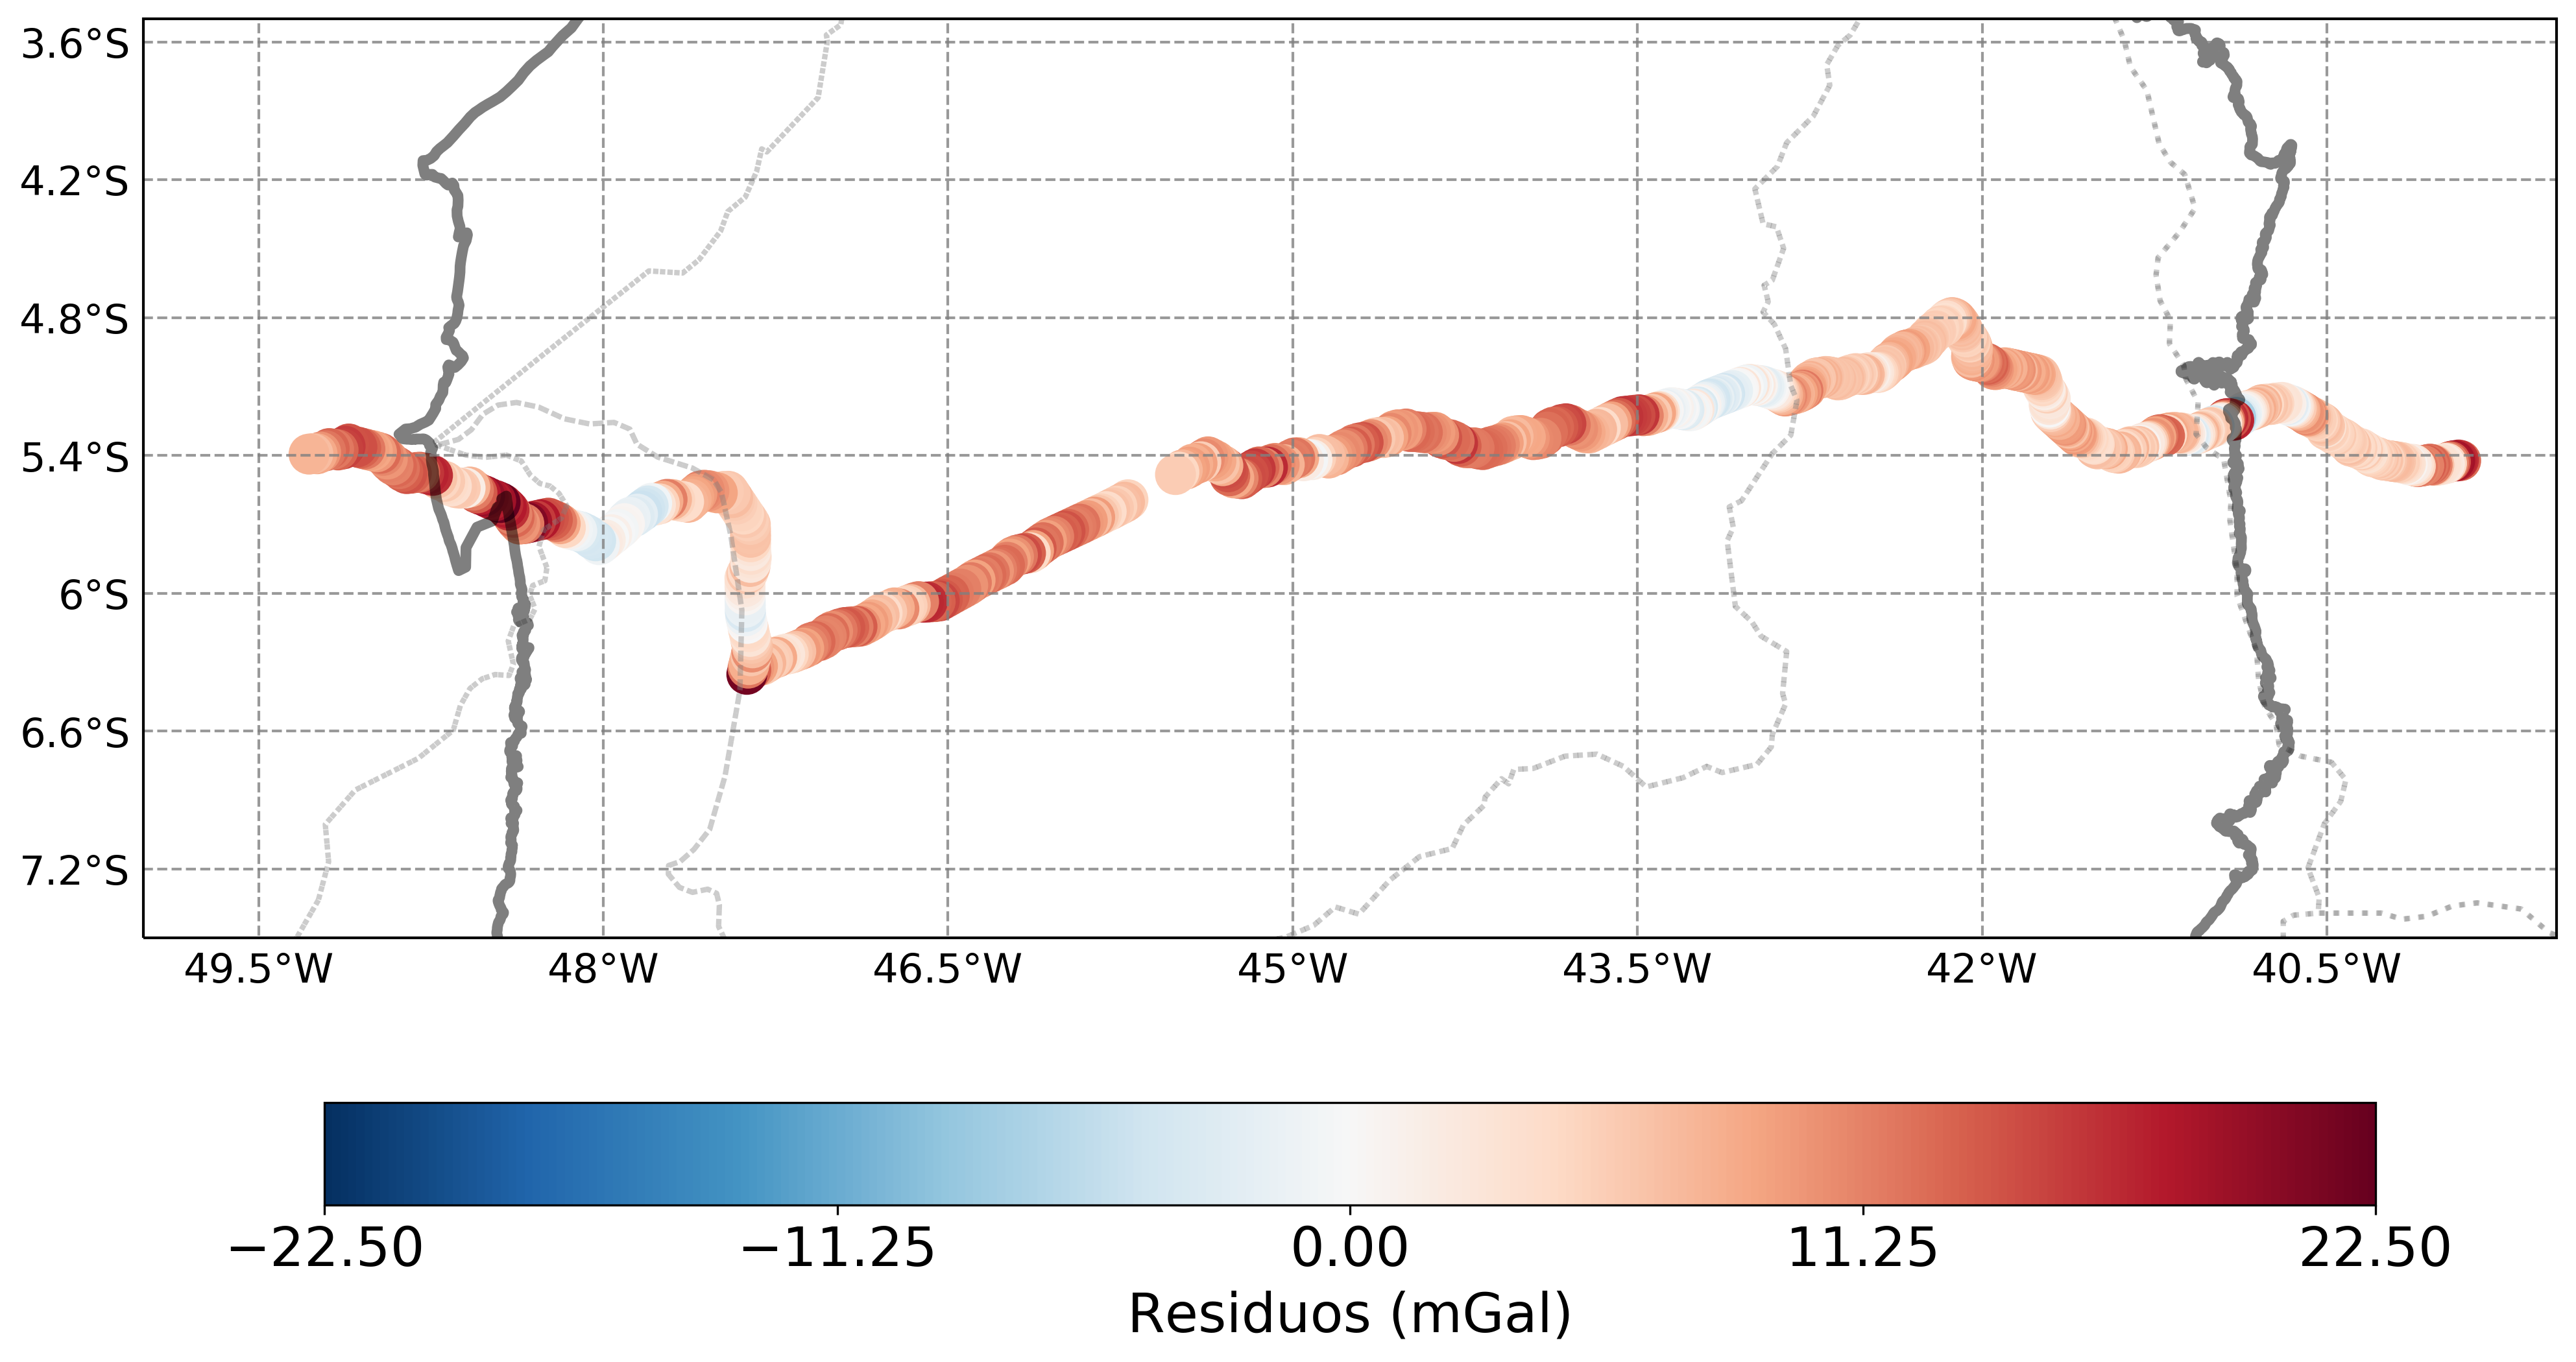
\includegraphics[scale=0.37]{figs/perfil residuos.png}}
	\caption{Esquema comparativo de $\delta g$ observado, $\delta g$ predito e resíduos de $\delta g$. O contorno preto representa os limites da bacia do Parnaíba, e o contorno cinza, o limite dos estados.}
	\label{subfig:residuos_delta}
\end{figure}

Os resíduos de $\delta g$ apresentaram valores predominantemente positivos que se repetem com maior frequência entre as faixas branca e vermelha, segundo a escala de cores, que corresponde à variação $0$ a $\approx15$ mGal. Esta análise também leva à hipótese de que os dados preditos estão subestimados em relação aos observados. É provável que uma das causas também possa ser o truncamento dos harmônicos esféricos. No entanto, uma combinação de fatores também pode ser especulada. Lembrando que como o modelo \textit{EIGEN-6C4} é composto pela combinação de dados de diferentes origens, é relevante considerar que possa ter havido uma inclusão menos significativa de dados terrestres, uma vez que há uma baixa cobertura de dados no território brasileiro em comparação com outras localidades do planeta. Sendo assim, é possível pensar que o modelo \textit{EIGEN-6C4} seja menos acurado em determinadas regiões do globo, como na Bacia do Parnaíba. Para analisar estas subestimativas foi gerado o histograma da Figura \ref{subfig:histograma_delta}.a com média igual a $7.18$ $mGal$ e desvio padrão de $4.81$ $mGal$, onde se constata  resíduos predominantemente positivos. Essa análise corrobora a hipótese de dados calculados a partir do modelo estarem subestimados e evidenciam um erro de tendência. Foi gerado o gráfico de correlação da Figura \ref{subfig:histograma_delta}.b com valores de $\delta g$ observados e preditos para o levantamento, onde é possível constatar uma forte correlação  linear com $R^{2}$ igual à $0.92$, muito embora haja uma maior dispersão dos pontos em comparação com a análise feita para as altitudes geométricas (Figura \ref{subfig:histograma_h}.b). Além disso, nota-se que há uma densificação maior de pontos para valores negativos do que para positivos. 

\begin{figure}[H]
	\centering
	\subfloat[Histograma dos resíduos de $\delta g$, onde é possível observar um comportamento na média de $7.18$ $mGal$ e desvio padrão de $4.81$. A linha vermelha pontilhada corresponde ao hisograma de resíduos de $\delta g$ teórico, considerando uma distribuição gaussiana.]{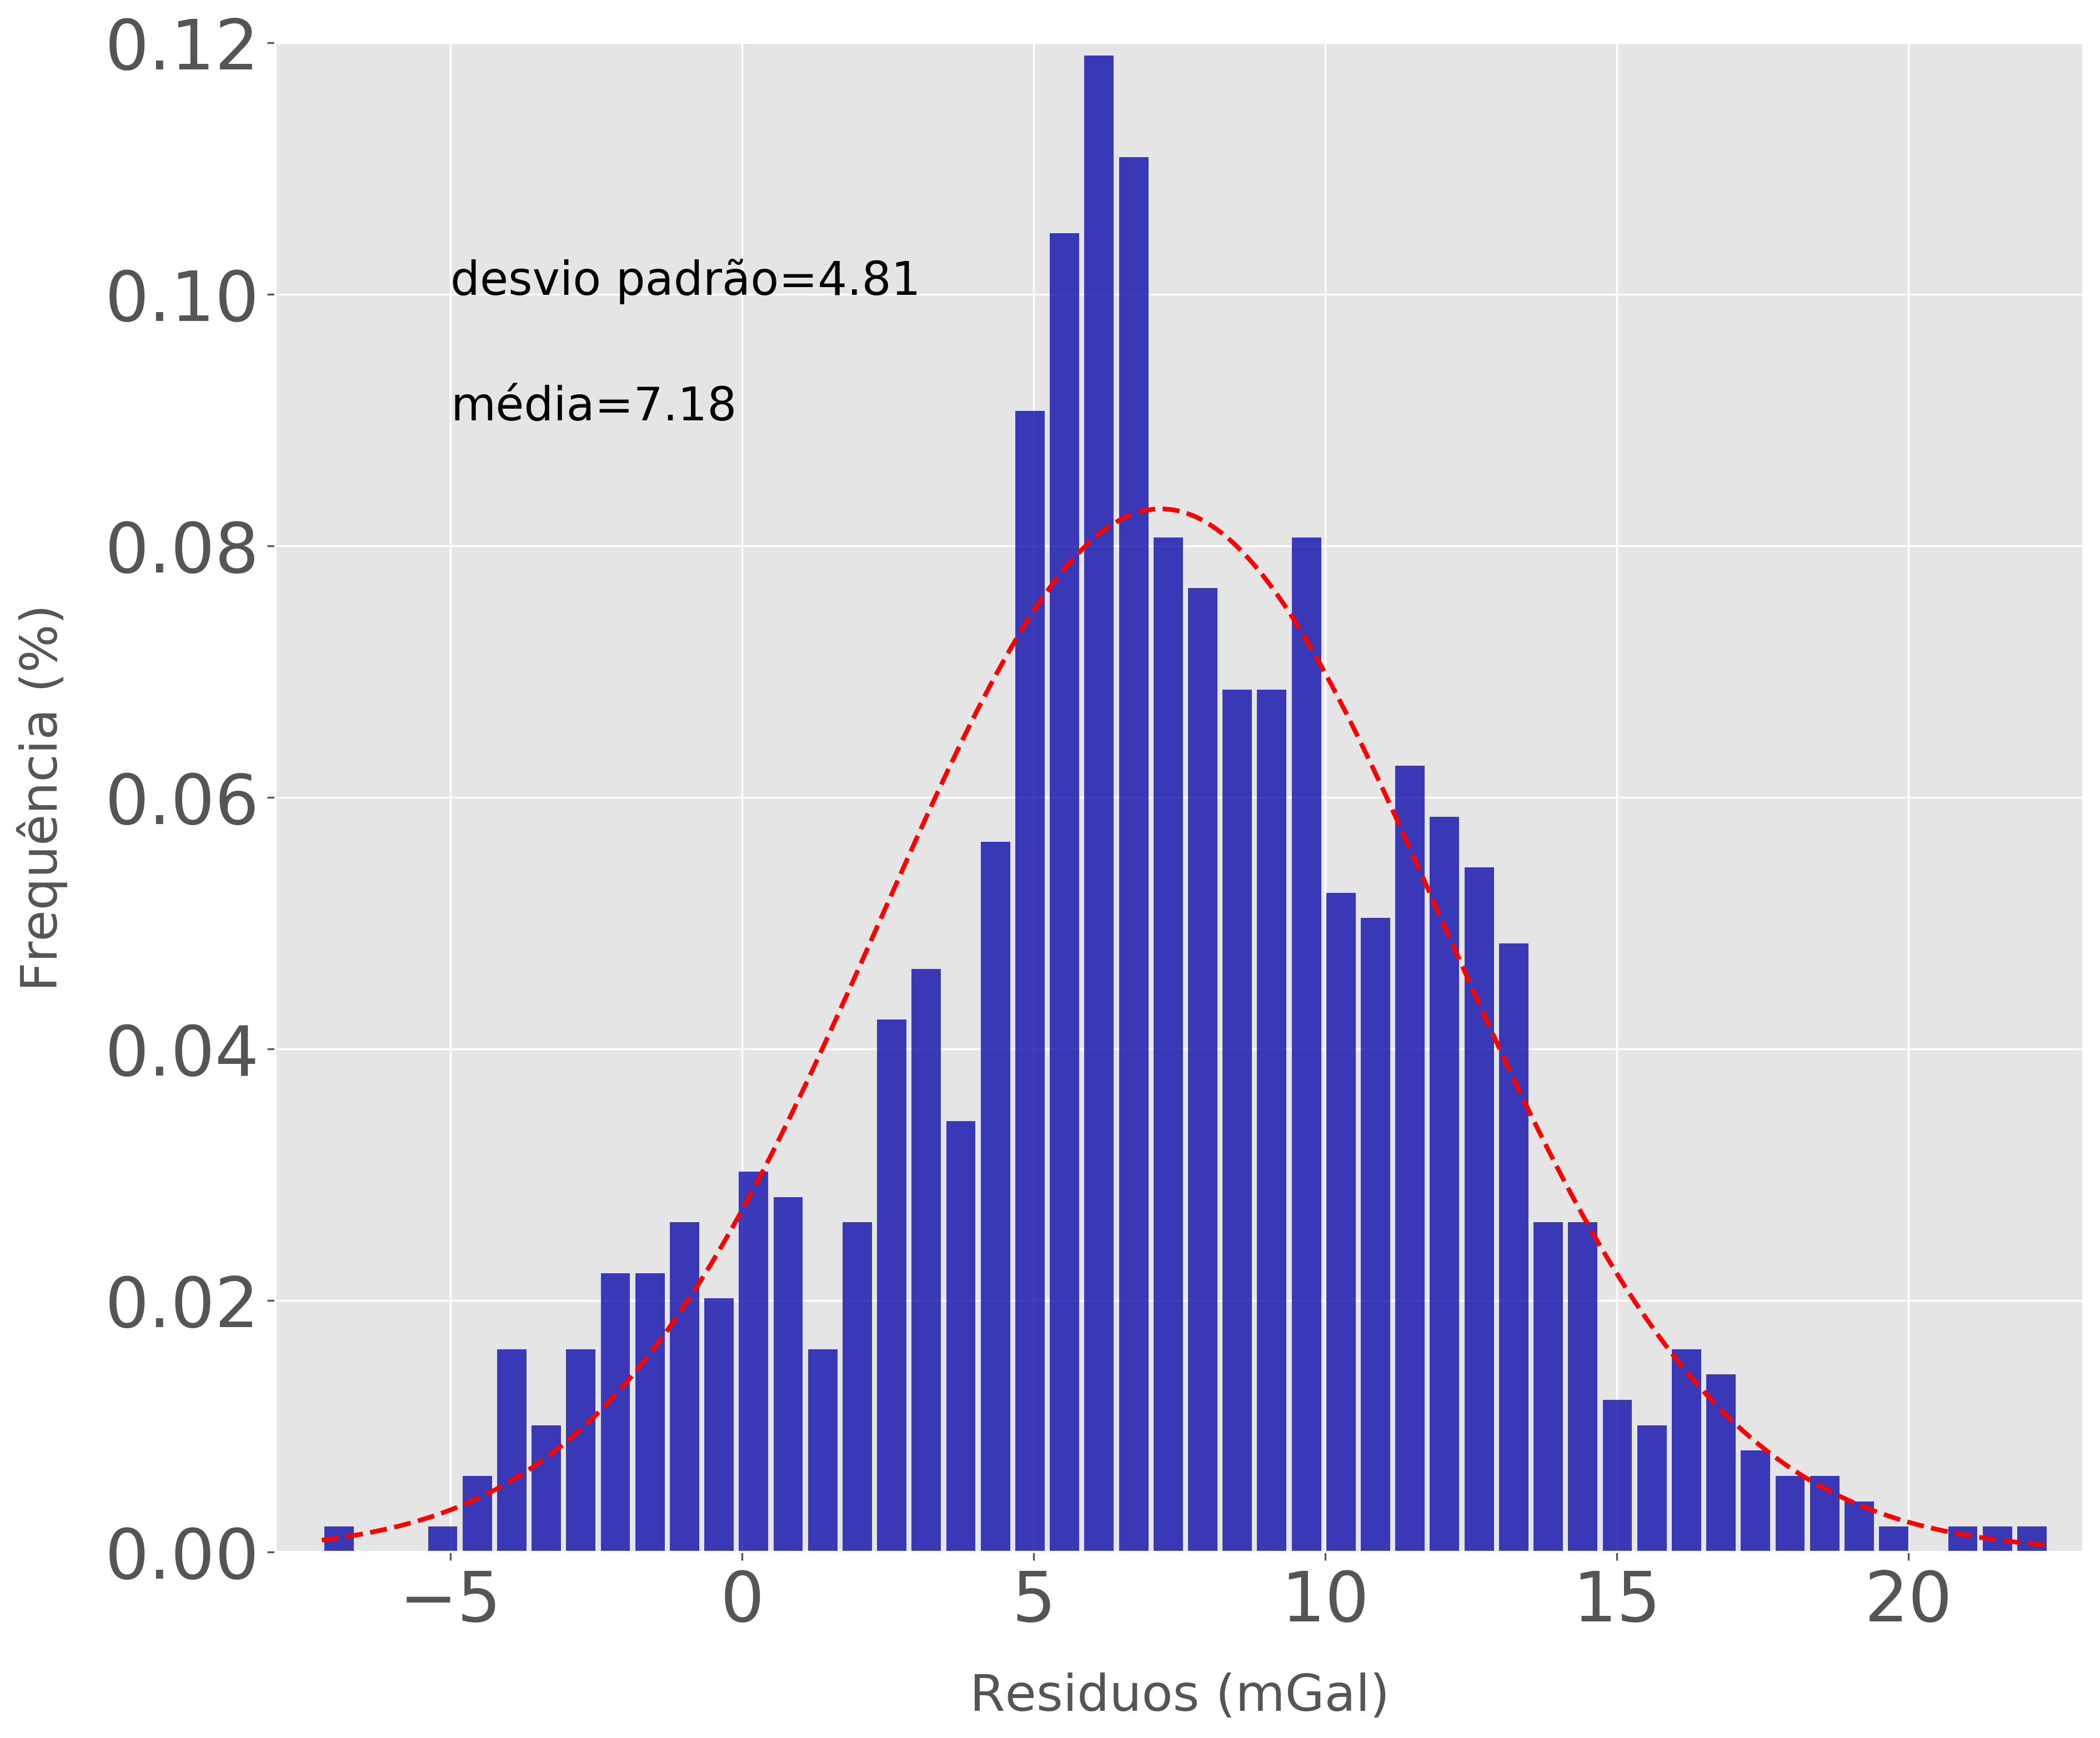
\includegraphics[scale=0.245]{figs/histograma_residuos_delta.png}}
	\
	\,\,\subfloat[Gráfico de dispersão de $\delta g$, observado e predito, com ajuste linear representado pela reta vermelha com $R^{2}$ igual a $0.92$]{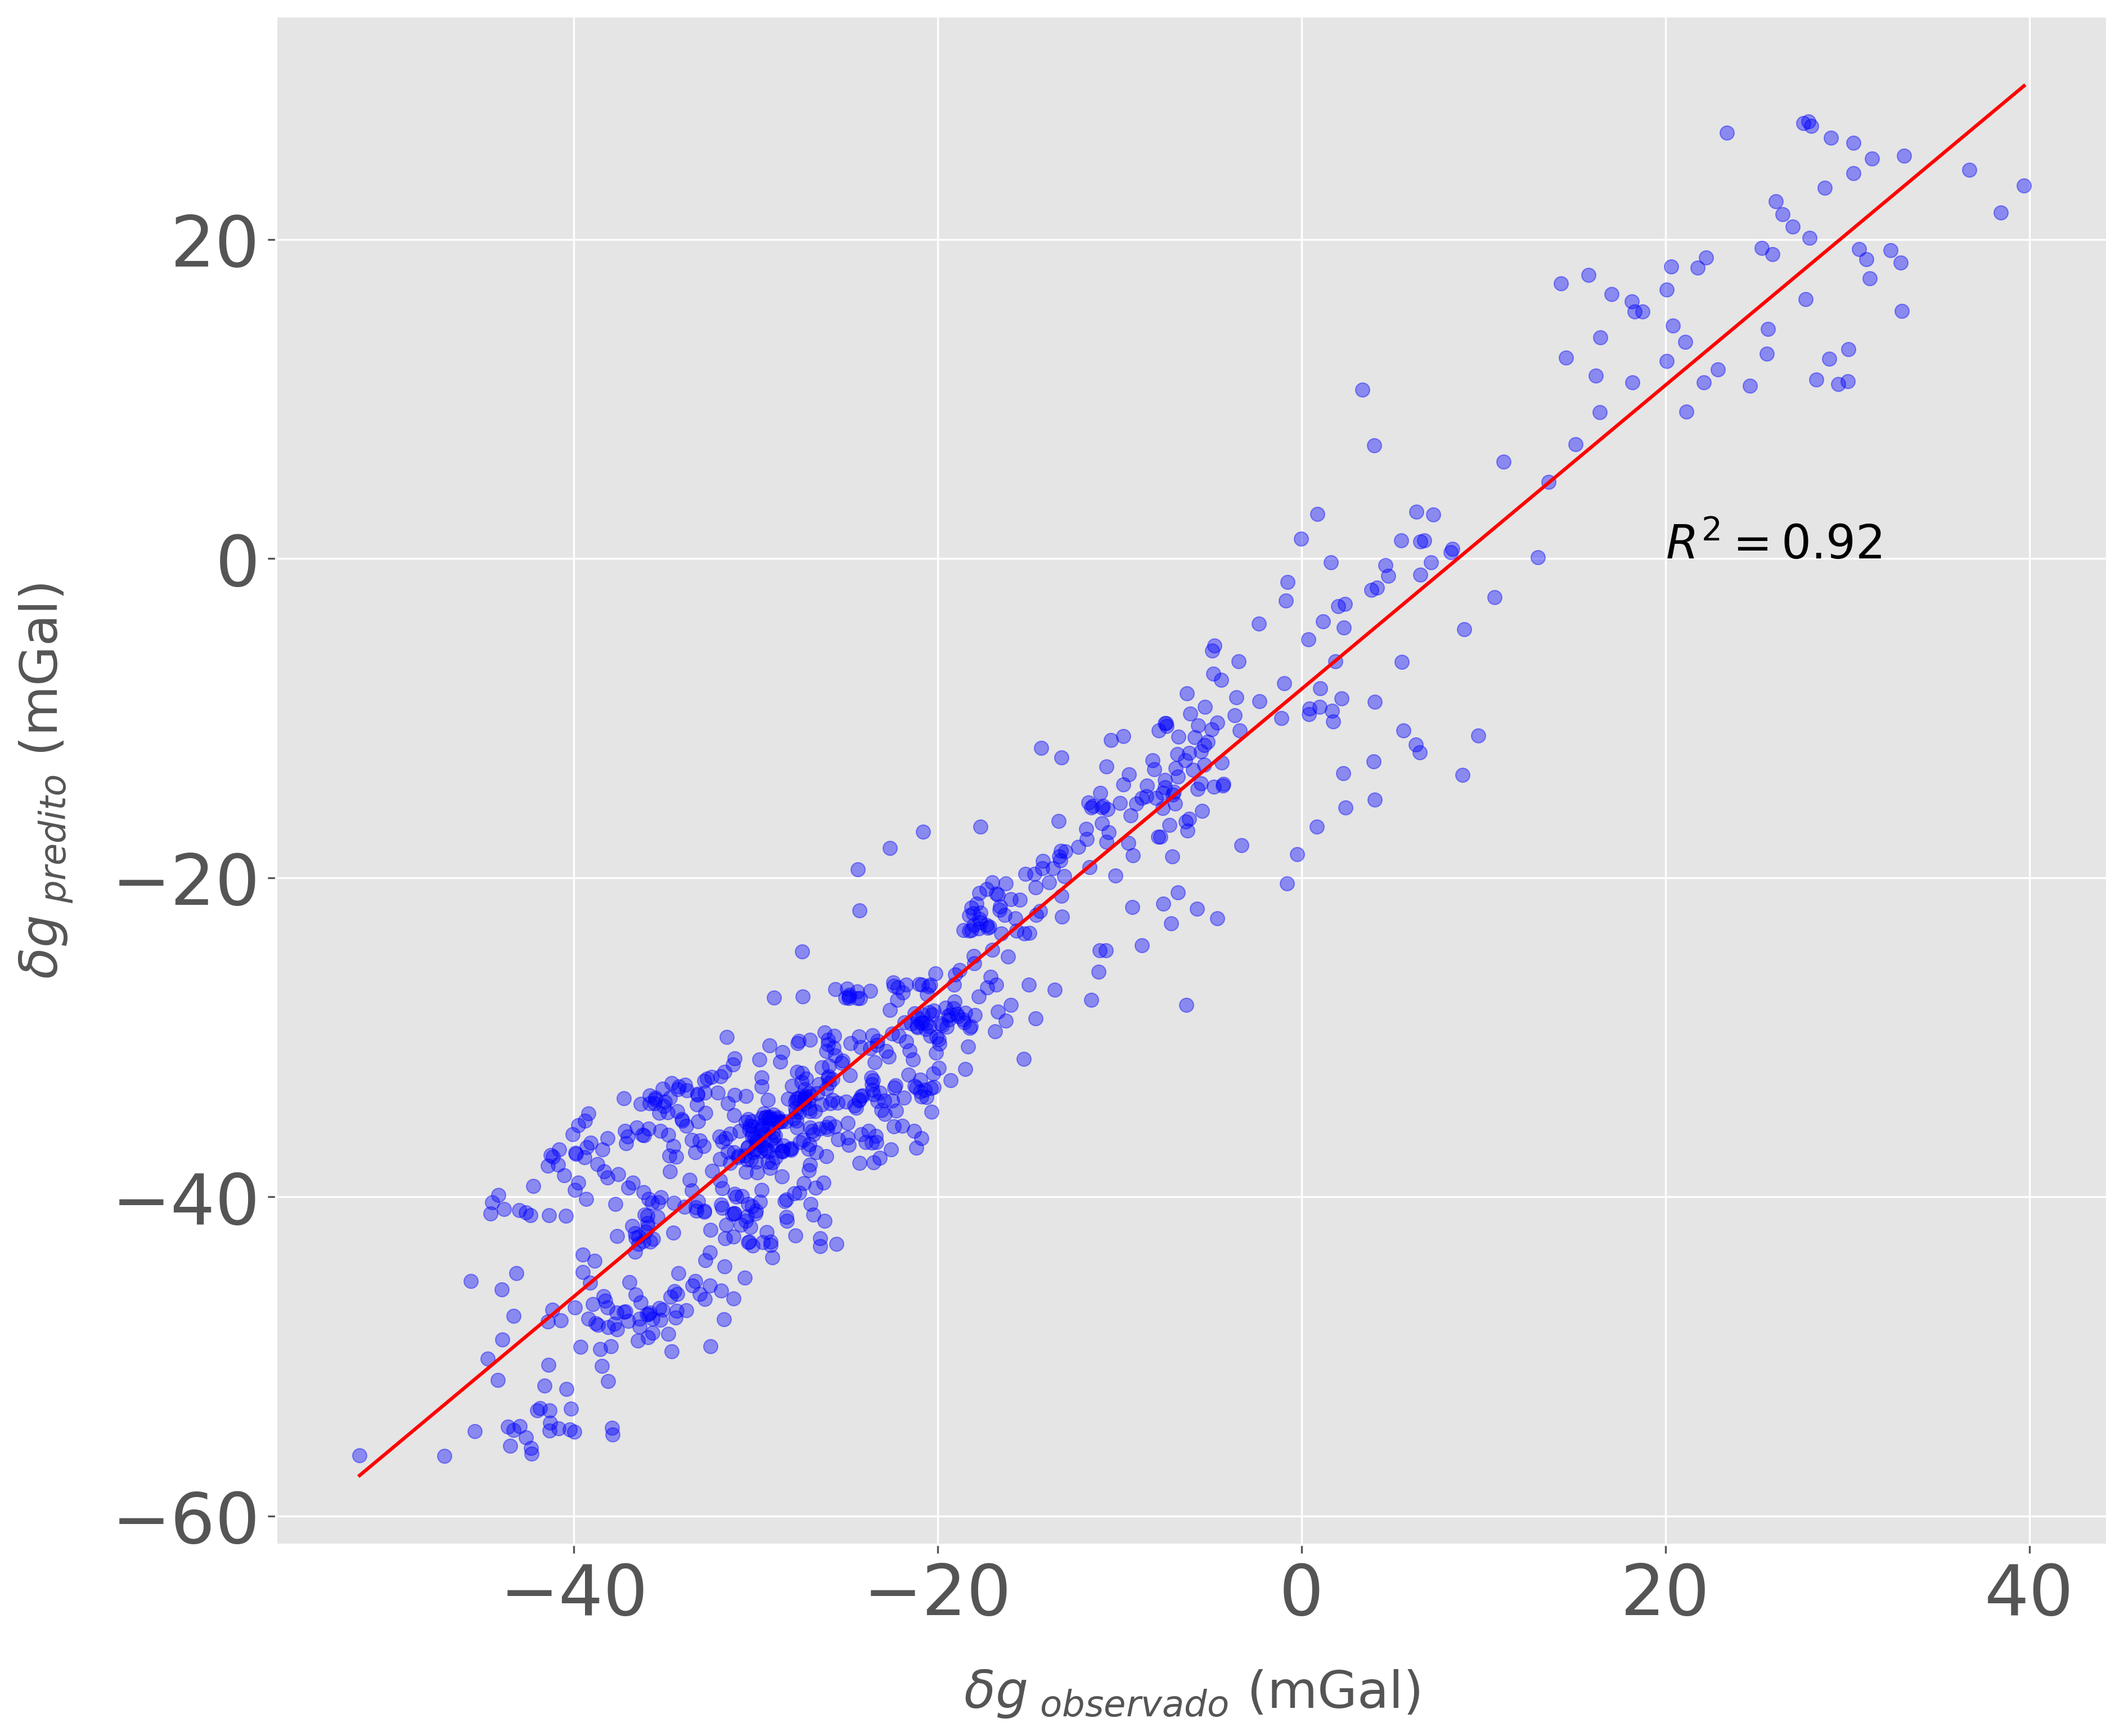
\includegraphics[scale=0.245]{figs/dispersao delta obs x pred.png}} 
	\caption{Esquema comparativo com histograma de resíduos de $\delta g$ ao lado do gráfico de correlação de $\delta g$ predito e $\delta g$ observados.}
	\label{subfig:histograma_delta}
\end{figure}

\section{Análise de dispersão complementar}

Foram gerados gráficos de correlação para complementar as análises anteriores a partir de $h$ e $\delta g$, e os resíduos de $h$ com resíduos de $\delta g$. A Figura \ref{subfig:h_delta}.a apresenta a correlação entre $\delta g$ observado e $h$ observada. Constata-se uma boa correlação linear entre as grandezas supracitadas, evidenciada pelo $R^{2} = 0.64$. Adicionalmente, observa-se uma maior dispersão para os menores valores de altitude e distúrbio de gravidade. Esse padrão não se repete para os maiores valores apresentados no gráfico, em decorrência da amostragem dos dados. É comum a associação de que regiões cujas altitudes são elevadas, possuem valores de gravidade menores. No entanto, o gráfico reflete o oposto, ou seja, em regiões de maiores altitudes, observamos distúrbios de gravidade igualmente elevados. E mais: são nestas regiões que a relação $h \times \delta g$ sofre menos dispersão. Pode-se inferir, portanto, que nessas regiões existe maior heterogeneidade de rochas em subsuperfície. As Figuras \ref{subfig:h_delta}.b e \ref{subfig:h_delta.b}.a apresentam a correlação entre $\delta g$ predito com $h$ predita e $\delta g$ predito com $h$ observado, respectivamente. Assim como a Figura \ref{subfig:h_delta}.a, existe certo padrão de correlação linear ($R^{2} = 0.64$). As amplitudes apresentam maior dispersão (i.e. menor correlação), mas, é possível constatar que os coeficientes de determinação apresentam pouca variação. Nas Figuras \ref{subfig:h_delta}.a, \ref{subfig:h_delta}.b e \ref{subfig:h_delta.b}.a é possível observar o padrão de maior adensamento de dados em altitudes menores, dada a baixa amostragem dos dados, referenciada anteriormente. A Figura \ref{subfig:h_delta.b}.b apresenta a correlação entre resíduos de $\delta g$ e de $h$. É notório que não existe qualquer correlação linear, dado o padrão bastante dispersivo associado ao baixo $R^{2}$ igual a $0.13$.

\begin{figure}[H]
	\centering
	\subfloat[Gráfico de dispersão de $\delta g$ observados com $h$ observado, apresentando um índice de determinação de $0.64$]{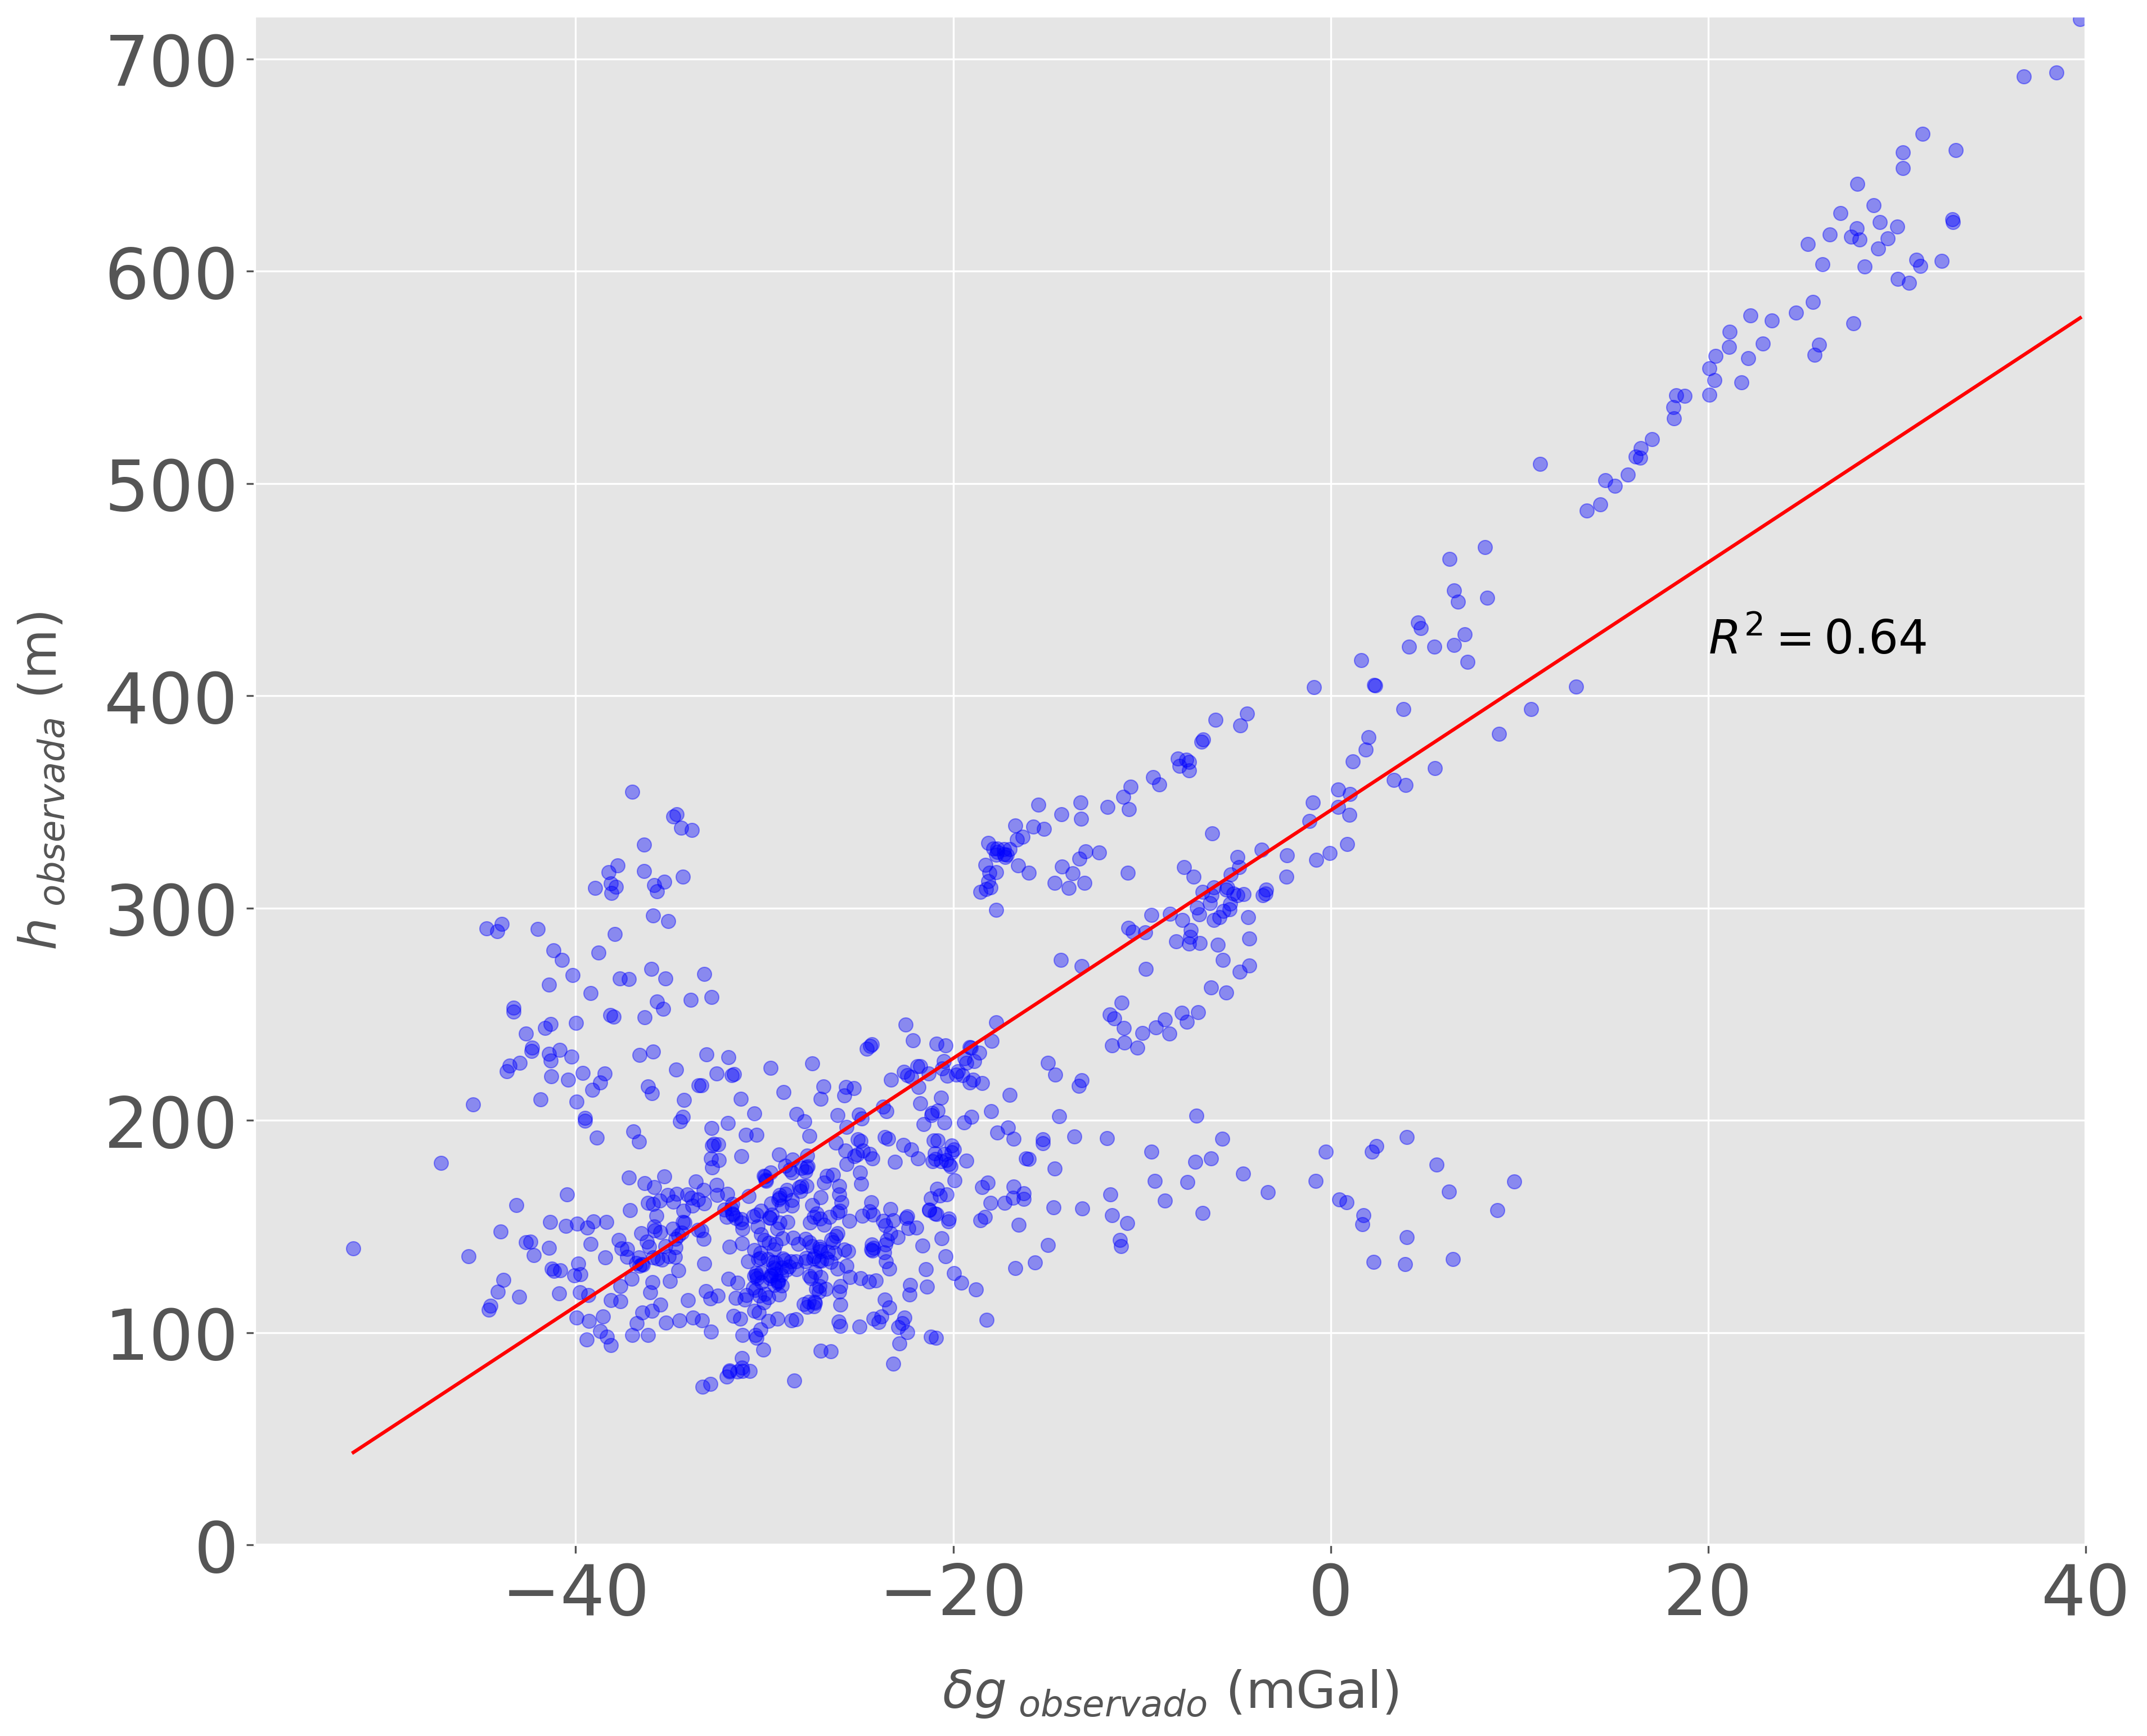
\includegraphics[scale=0.24]{figs/dispersao delta obs x h obs.png}}
	\
	\,\subfloat[Gráfico de dispersão de $\delta g$ preditos com $h$ predito, apresentando um índice de determinação de $0.67$]{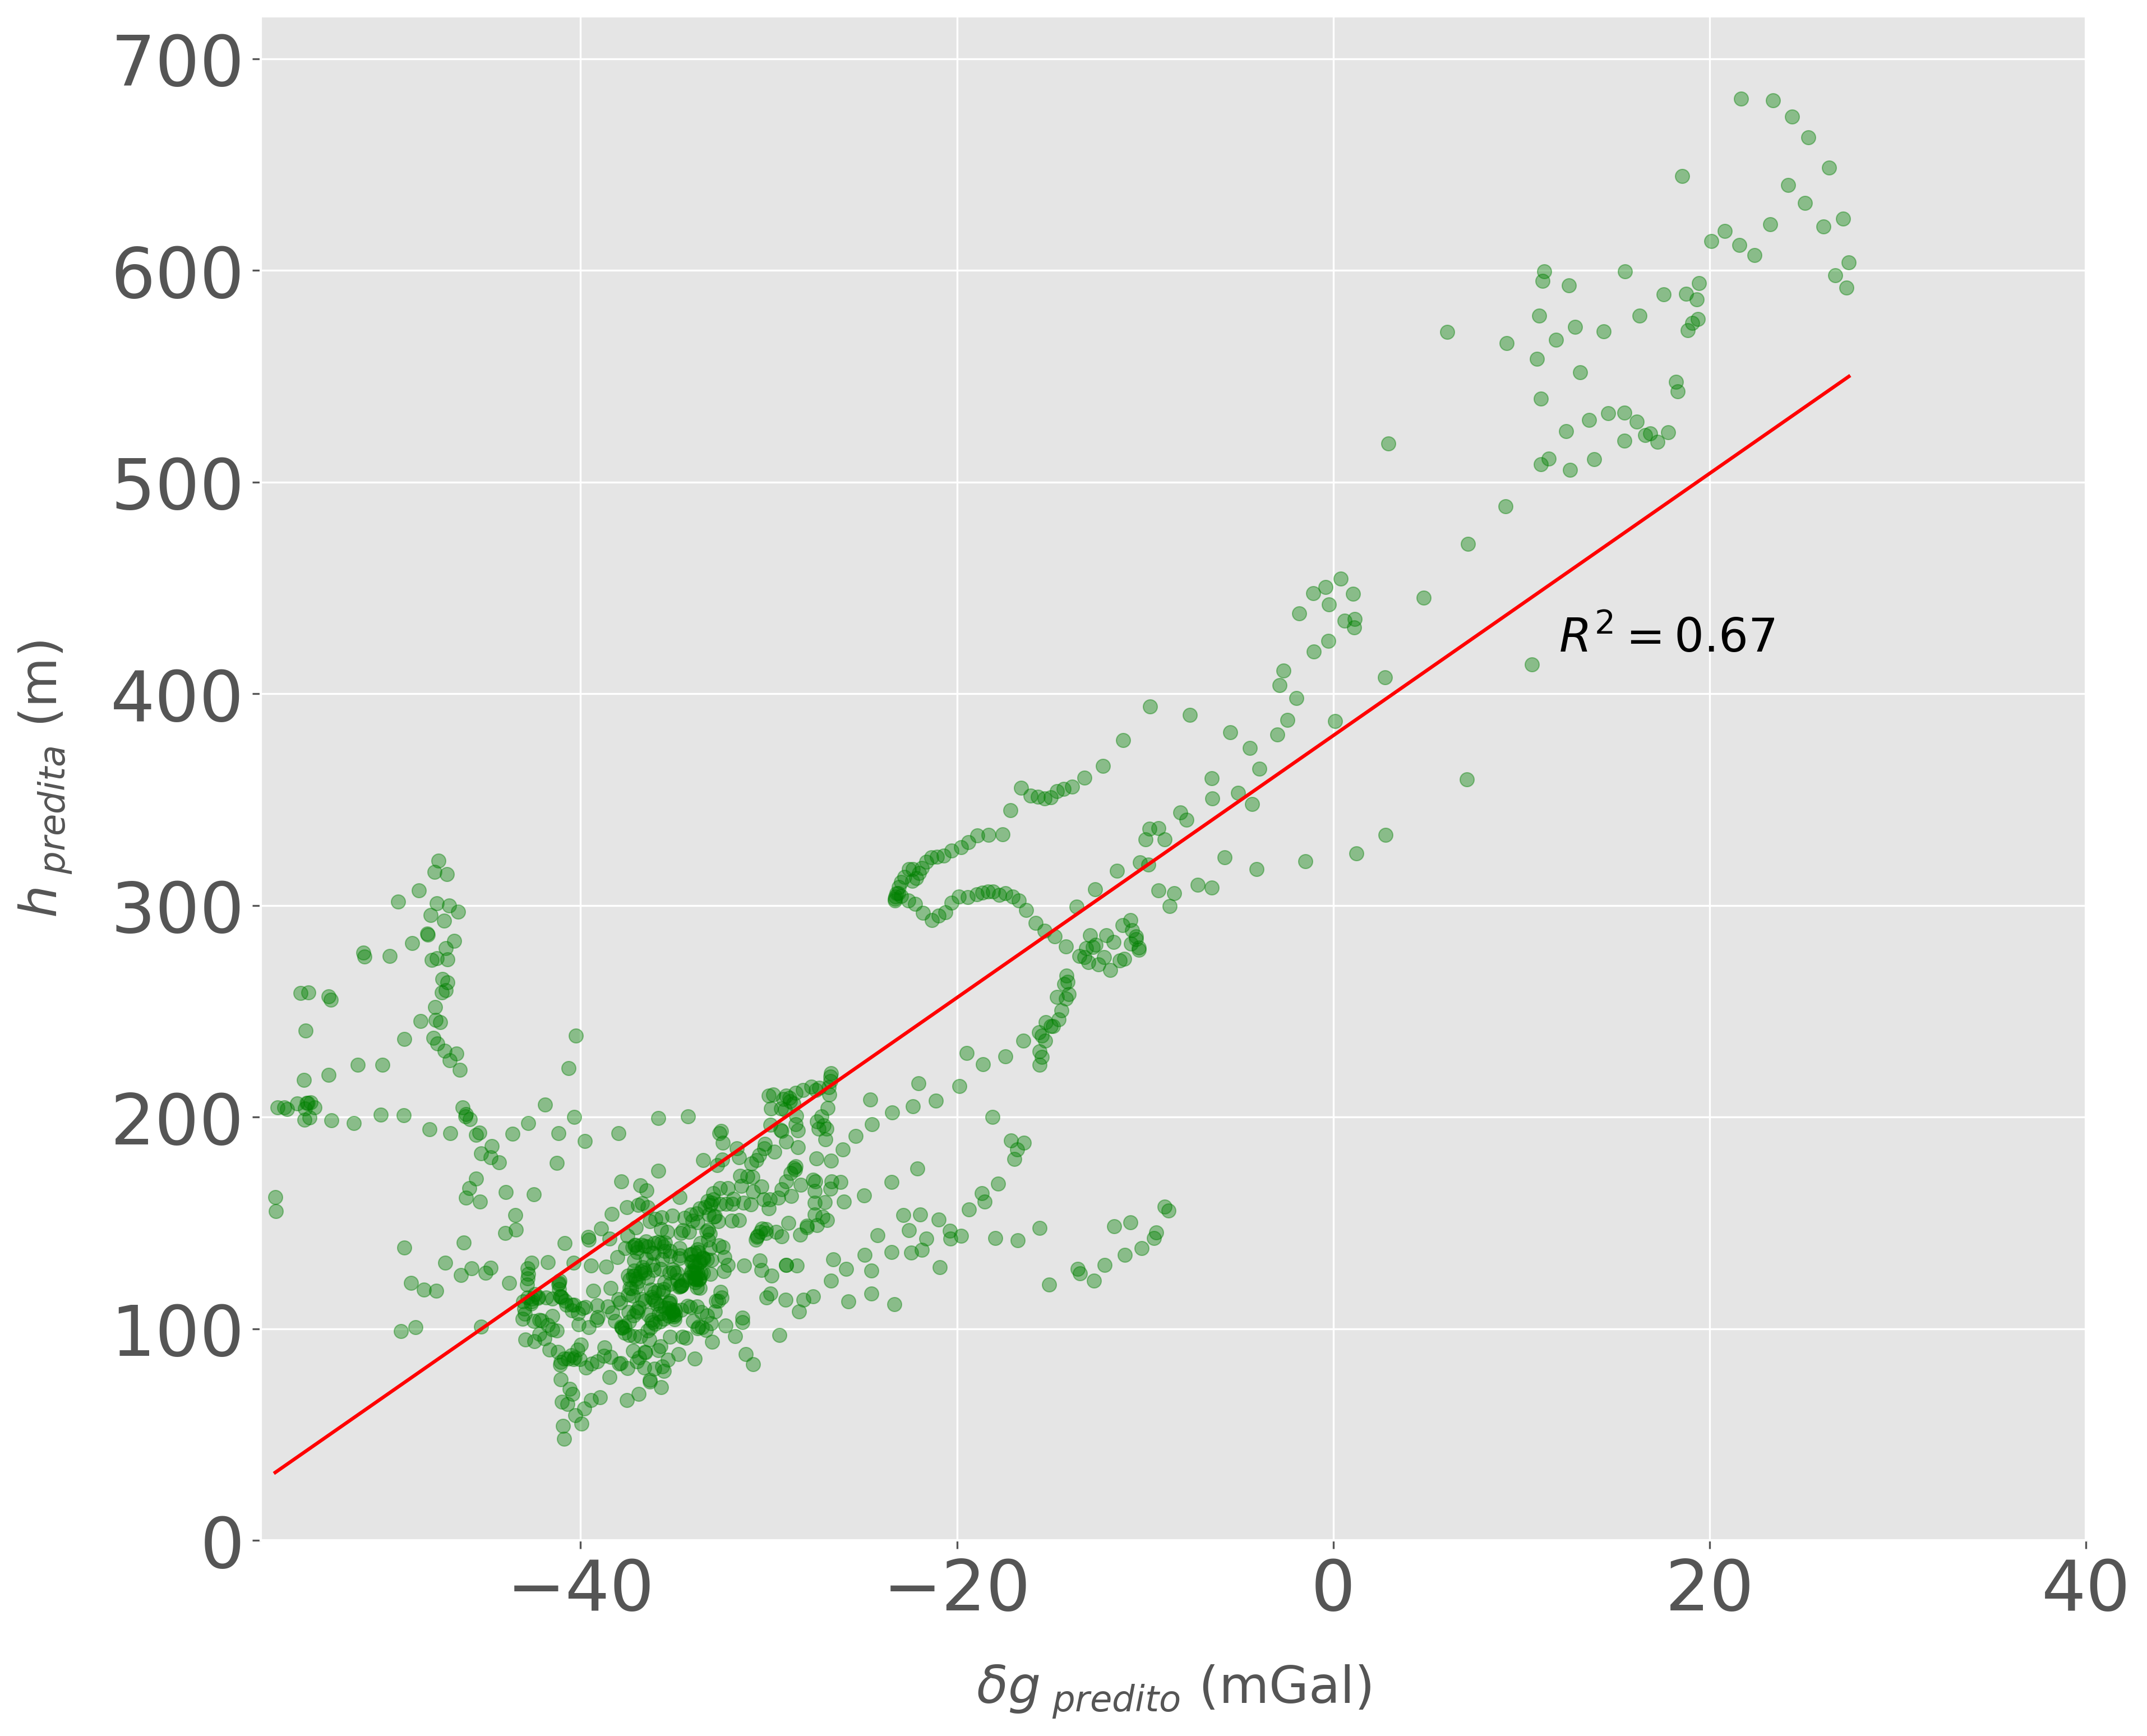
\includegraphics[scale=0.24]{figs/dispersao delta pred x h pred.png}} 
	\caption{Esquema comparativo com gráficos de correlação entre $\delta g$ e $h$. A linha vermelha corresponde ao ajuste linear entre os parâmetros dos gráficos.}
	\label{subfig:h_delta}
\end{figure}
\begin{figure}[H]
	\centering
	\subfloat[Gráfico de dispersão de $\delta g$ predito com $h$ observado, apresentando um índice de determinação de $0.64$]{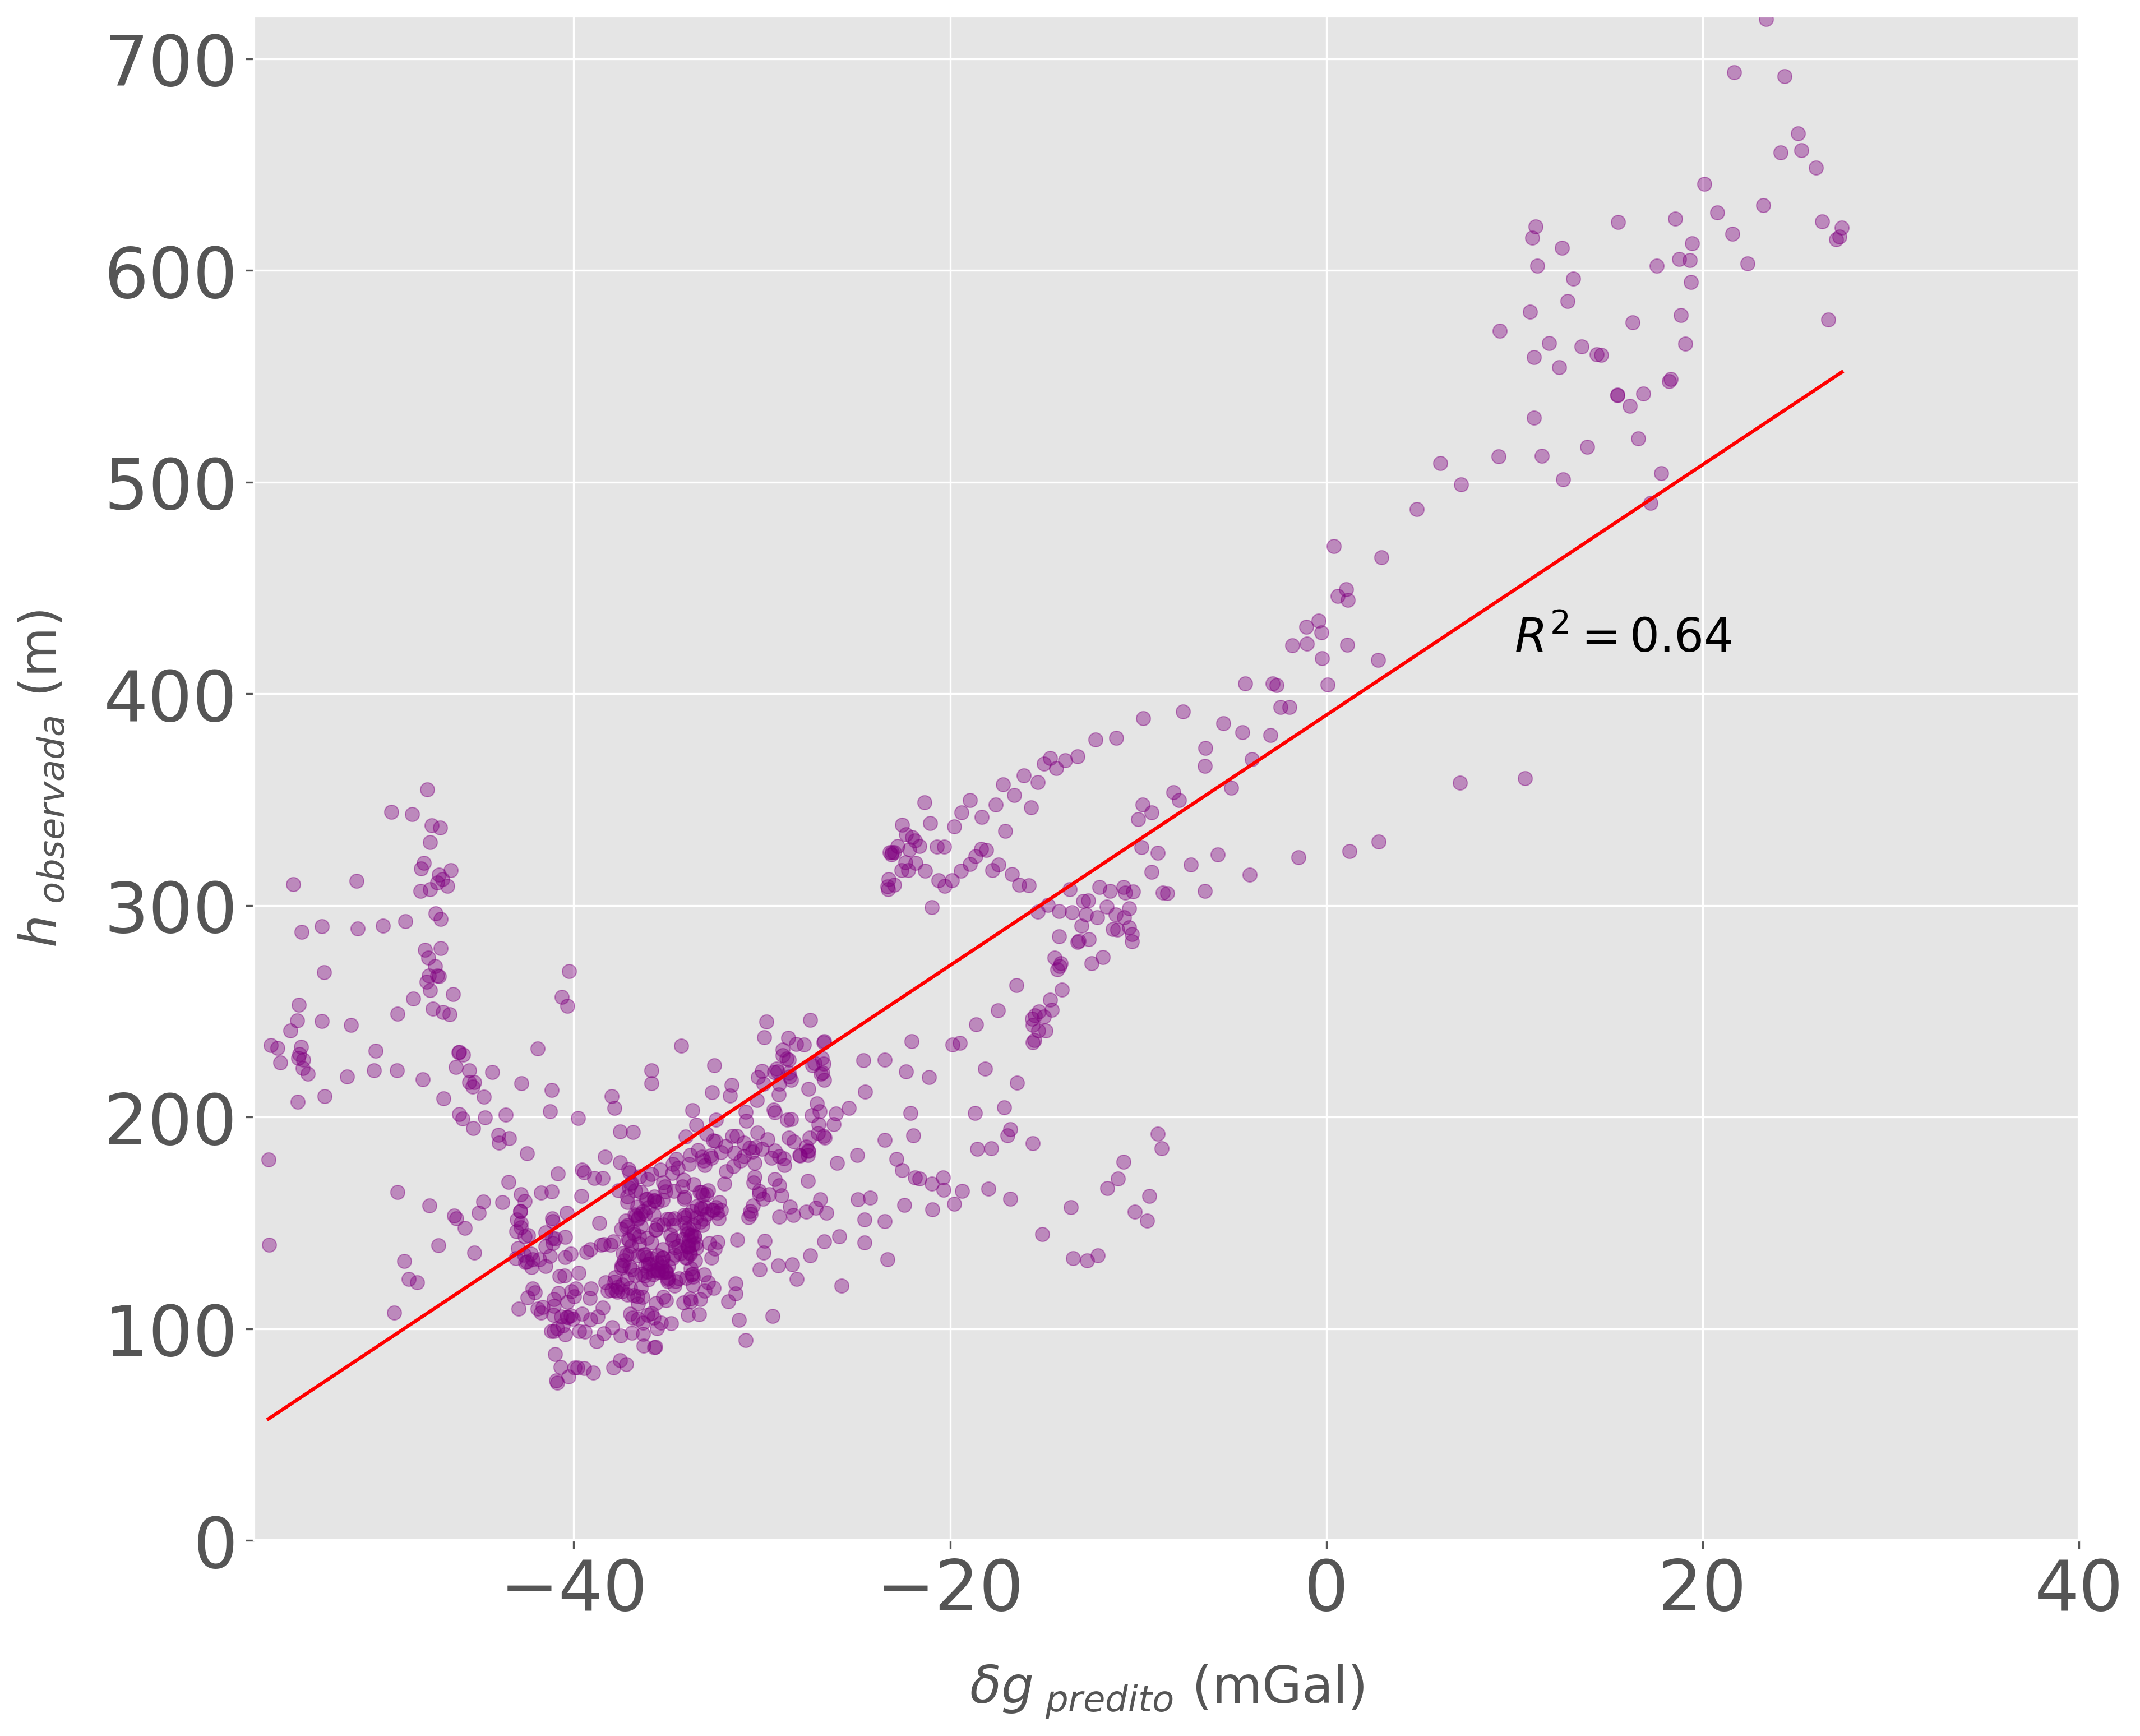
\includegraphics[scale=0.24]{figs/dispersao delta pred x h obs.png}}
	\	
	\subfloat[Gráfico de dispersão comparando os resíduos de $h$ com os resíduos de $\delta g$, apresentando um índice de determinação de $0.13$]{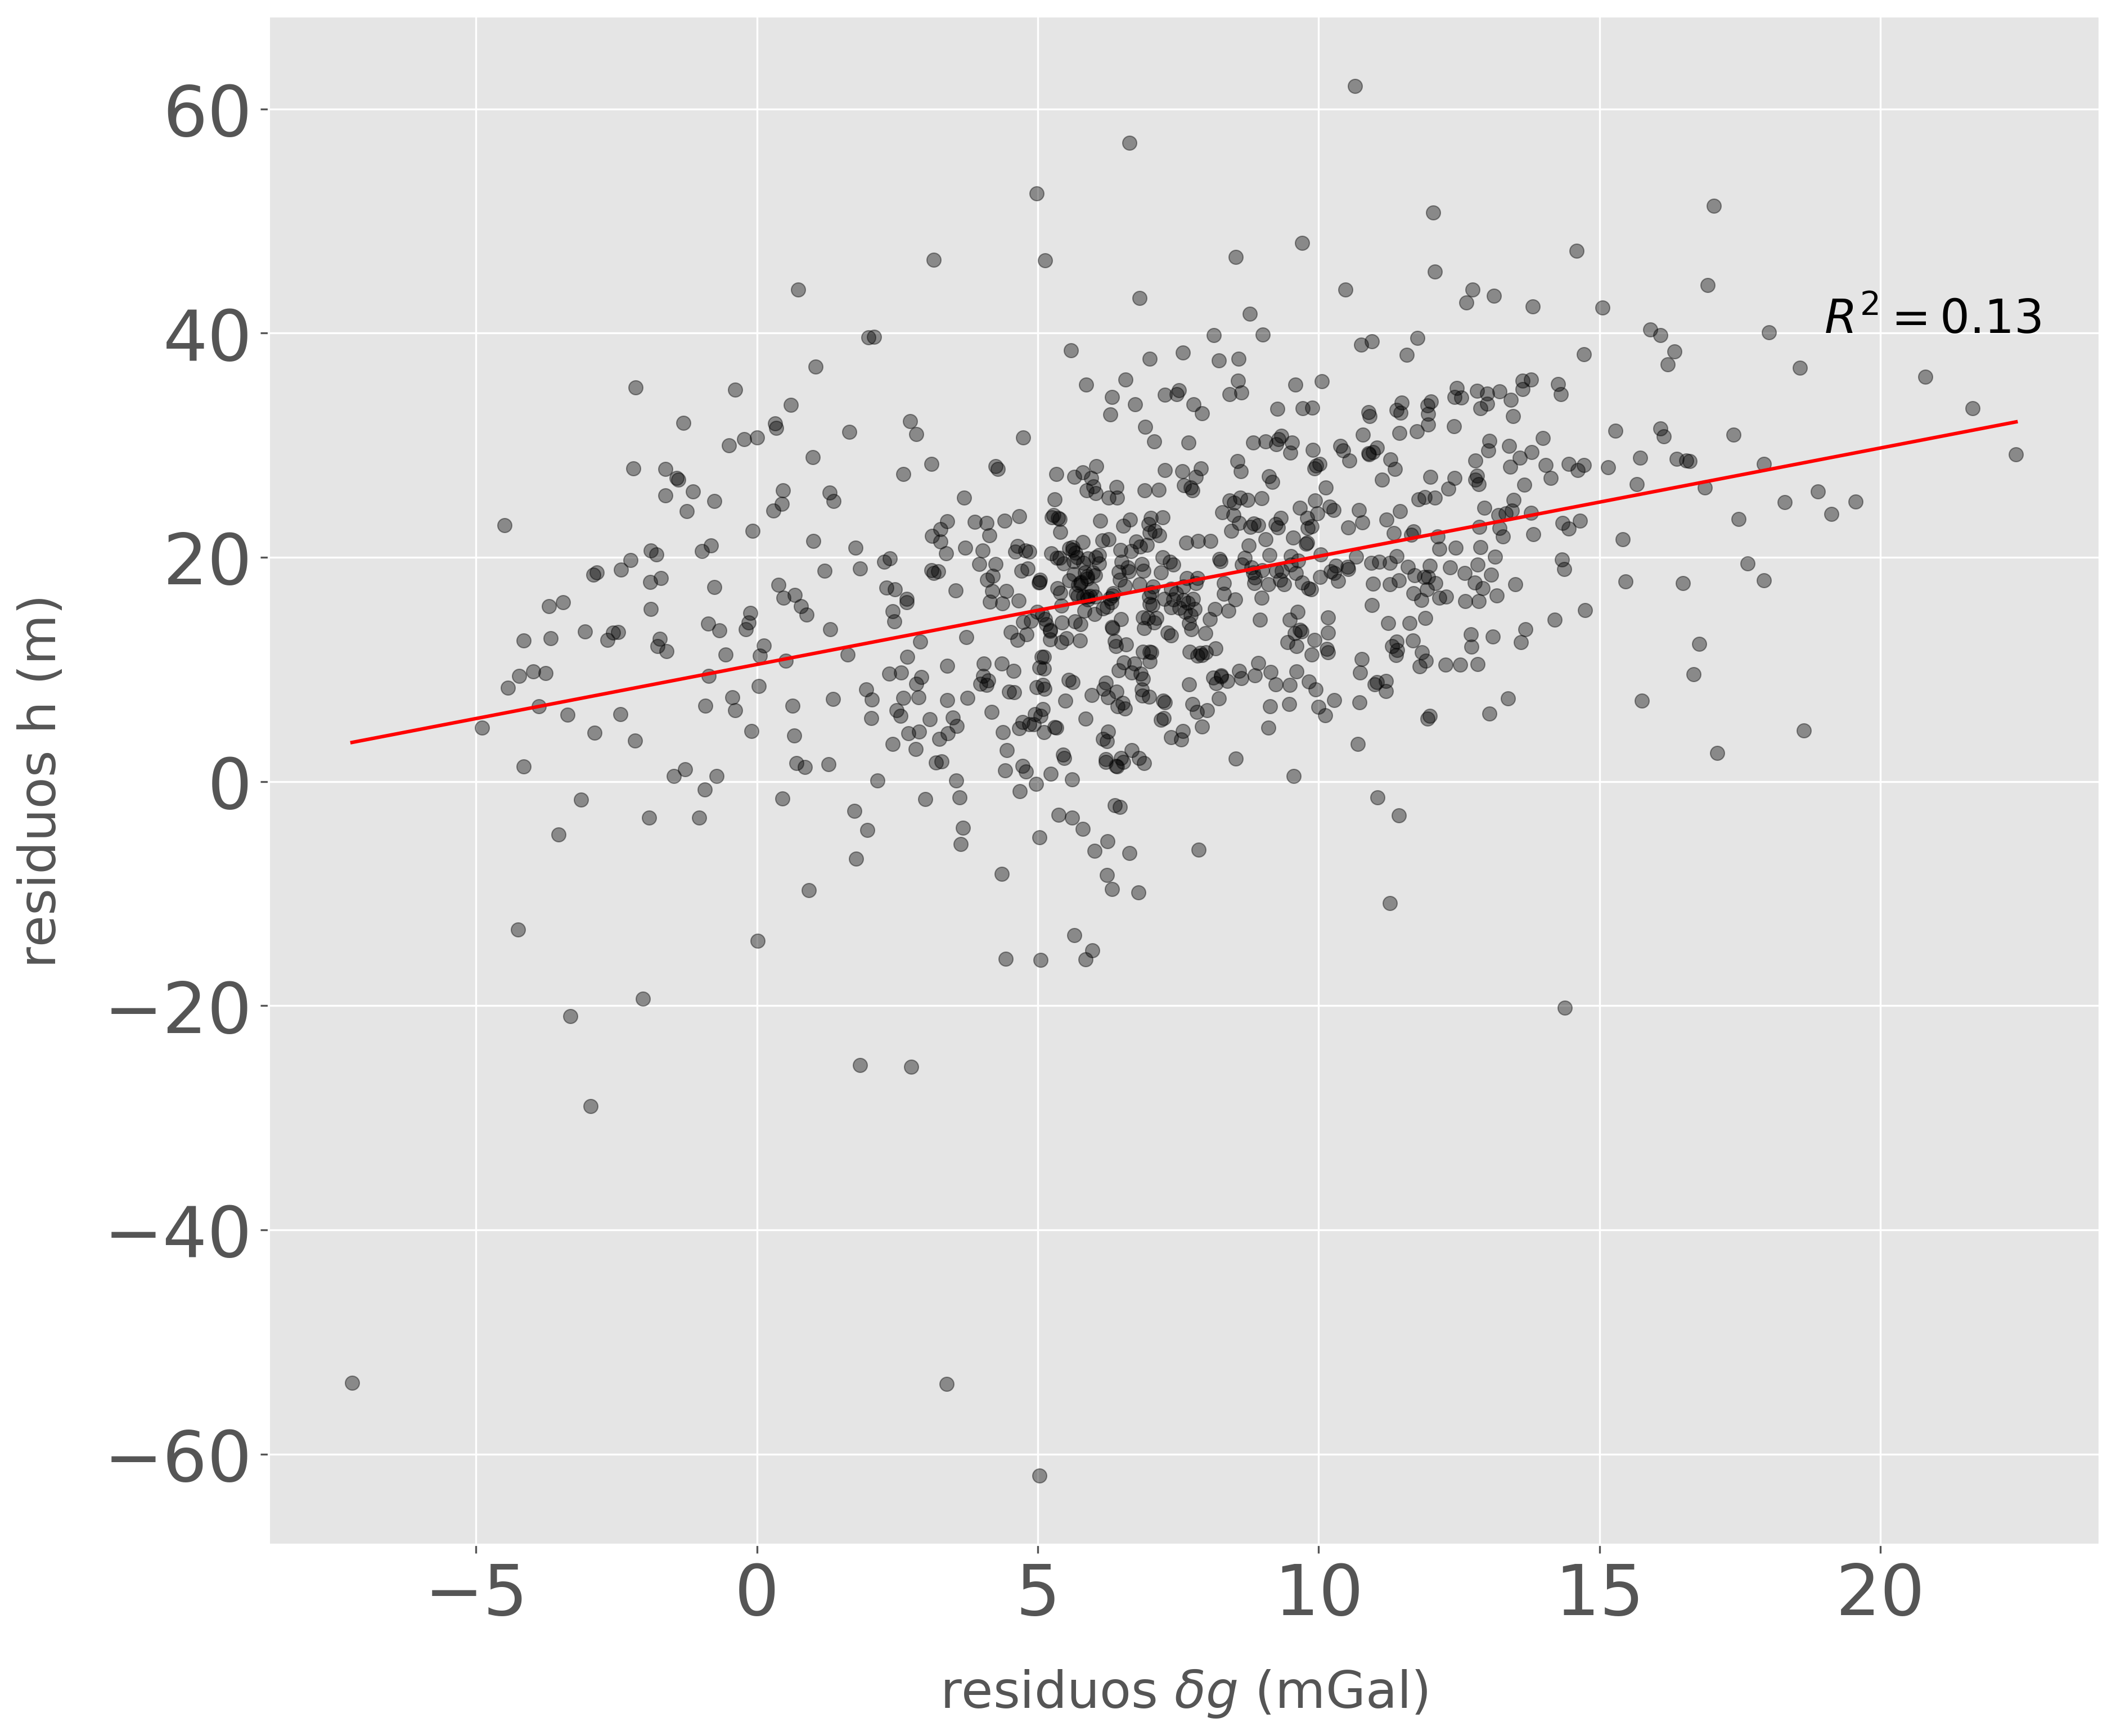
\includegraphics[scale=0.24]{figs/dispersao residuos.png}}
	\caption{Esquema comparativo com gráficos de correlação entre $\delta g$ predito e $h$ observado, e resíduos de $h$ com resíduos de $\delta g$. A linha vermelha corresponde ao ajuste linear entre os parâmetros dos gráficos.}
	\label{subfig:h_delta.b}
\end{figure}

